\pdfoutput=1

\documentclass[sigconf,screen=true,anonymous]{acmart} 
% \documentclass[sigconf,screen=true]{acmart} 

%%%%%

% Copyright
%\setcopyright{none}
%\setcopyright{acmcopyright}
%\setcopyright{acmlicensed}
\setcopyright{rightsretained}
%\setcopyright{usgov}
%\setcopyright{usgovmixed}
%\setcopyright{cagov}
%\setcopyright{cagovmixed}

% DOI
% \acmDOI{10.475/123_4}
% ISBN
% \acmISBN{123-4567-24-567/08/06}

\acmConference[WWW 2019]{The Web Conference 2019:  The 28th International World Wide Web Conference}{May 13-17, 2019}{San Francisco}
\acmYear{2019}
\copyrightyear{2019}

\settopmatter{printfolios=false,printacmref=true}
\fancyhead{}

% Space hacks
\clubpenalty=10000
\widowpenalty=10000
\usepackage[subtle, wordspacing=normal, tracking=normal, bibnotes, charwidths=normal, leading, indent, lists, paragraphs=normal, mathspacing=normal, bibliography=normal]{savetrees}
\looseness=-1

\usepackage{hyperref}
\usepackage{booktabs} % For formal tables
\usepackage{subfig}
\usepackage[skip=0pt]{caption}
\usepackage{graphicx}
\usepackage{paralist}
\usepackage{enumitem}
\usepackage{acronym}
\usepackage{amsmath}
\newcommand{\todo}[1]{\textcolor{red}{TODO: #1}}
%\newcommand{\im}[1]{\textcolor{blue}{IM: #1}}
%\newcommand{\mdr}[1]{\textcolor{cyan}{#1}}
\acrodef{LTR}{learning to rank}
\acrodef{ViTOR}{\textit{Visual learning TO Rank}}
\acrodef{SERP}{search engine result page}

\newcommand{\datasetname}{\ac{ViTOR}}
\newcommand{\modelname}{\ac{ViTOR}}
\newcommand{\OK}{@{\mbox{}\hspace*{.25cm}}}

\title{ViTOR: Learning to Rank Web Pages Based on Visual Features}
% \subtitle{An Improved Method and a Dataset}

\author{Bram van den Akker}
\orcid{}
\affiliation{%
  \institution{University of Amsterdam}
  \city{Amsterdam} 
  \country{The Netherlands}
}
\email{bram.vandenakker@student.uva.nl}

\author{Ilya Markov}
\orcid{}
\affiliation{%
  \institution{University of Amsterdam}
  \city{Amsterdam} 
  \country{The Netherlands}  
}
\email{i.markov@uva.nl}

\author{Maarten de Rijke}
\orcid{0000-0002-1086-0202}
\affiliation{%
   \institution{University of Amsterdam}
   \city{Amsterdam} 
   \country{The Netherlands}
}
\email{derijke@uva.nl}

% The default list of authors is too long for headers.
\renewcommand{\shortauthors}{B. van den Akker et al.}

\begin{document}

%Web page \ac{LTR} based on visual features is a method of ranking (textual) web pages for a query using their visual appearance as (additional) features.  
%
%In this work we improve web page \ac{LTR} based on visual features, a method of ranking web pages for a query using their visual appearance as (additional) features. 
%
%\mdr{In \ac{LTR} web pages using visual features one uses the visual appearance of web pages as (additional) features to rank (textual) web pages in response to a query.}
\begin{abstract}
Features learned from the visual appearance of a web page can help to improve \ac{LTR} performance. 
We introduce the \modelname~model, a multimodal architecture that can be used to combine both visual features and content features in order to create strong \ac{LTR} features. 
We demonstrate the \modelname~model performance by introducing two powerful feature extraction methods that significantly improve the performance of \ac{LTR} with visual features, namely: 
\begin{inparaenum}[(i)]
\item transfer learning from a pre-trained image recognition model, and
\item synthetic generated saliency heatmaps from web page snapshots.
\end{inparaenum}\ 
To support our work we also introduce and release the \datasetname~dataset, a rich and diverse dataset for \ac{LTR} with visual features.
\datasetname~consists of visual snapshots, non-visual features and relevance judgments for ClueWeb12 documents and the TREC Web Track.
The visual snapshots are rendered with both styling and images using the Wayback Machine and ClueWeb12 online rendering service.
Using \datasetname, we confirm that visual features can improve \ac{LTR} performance
and show the effectiveness of the newly introduced architecture and visual feature vectors.
% TODO maybe write something about the ability to use visual LTR cheaply.
\end{abstract}

%
% The code below should be generated by the tool at
% http://dl.acm.org/ccs.cfm
% Please copy and paste the code instead of the example below. 
%
% \begin{CCSXML}
% <ccs2012>
%  <concept>
%   <concept_id>10010520.10010553.10010562</concept_id>
%   <concept_desc>Computer systems organization~Embedded systems</concept_desc>
%   <concept_significance>500</concept_significance>
%  </concept>
%  <concept>
%   <concept_id>10010520.10010575.10010755</concept_id>
%   <concept_desc>Computer systems organization~Redundancy</concept_desc>
%   <concept_significance>300</concept_significance>
%  </concept>
%  <concept>
%   <concept_id>10010520.10010553.10010554</concept_id>
%   <concept_desc>Computer systems organization~Robotics</concept_desc>
%   <concept_significance>100</concept_significance>
%  </concept>
%  <concept>
%   <concept_id>10003033.10003083.10003095</concept_id>
%   <concept_desc>Networks~Network reliability</concept_desc>
%   <concept_significance>100</concept_significance>
%  </concept>
% </ccs2012>  
% \end{CCSXML}

% \ccsdesc[500]{Computer systems organization~Embedded systems}
% \ccsdesc[300]{Computer systems organization~Redundancy}
% \ccsdesc{Computer systems organization~Robotics}
% \ccsdesc[100]{Networks~Network reliability}


\keywords{Learning to rank, Visual features}


\maketitle

% !TEX root = cikm2018-visual-ltr.tex

\section{Introduction}
The design and appearance of a web are a determining factor for a user to examine a page or divert to another page~\cite{nielsen1999designing,nielsen2006f,pernice2017f,wang2014eye}.
Relatively little is known about the potential of visual features to help determine the perceived relevance of  a (web) page, in addition to content features such as BM25, quality indicators such as PageRank and behavioral features such as CTR.
Recently, \citet{fan2017learning} have introduced ViP, a \ac{LTR} model that uses a combination of both visual and content features.
Visual features are calculated from snapshots, which are in turn created by rendering web pages.
The authors demonstrate that adding these visual features helps to significantly improve the \ac{LTR} performance.

The work by \citet{fan2017learning} is important because it indicates that the visual appearance of a web page can have a significant impact on perceived utility, which opens a new direction in web search and \ac{LTR}.
However, there are several limitations in \cite{fan2017learning}.
First, the rendered web pages come from the the GOV2 collection~\todo{ref}.\footnote{\url{http://ir.dcs.gla.ac.uk/test_collections/gov2-summary.htm}}
This collection is limited in the sense that:
\begin{inparaenum}[(i)]
\item it solely contains web pages within the .gov domain crawled in 2004, i.e., somewhat outdated pages with a relatively narrow scope,
\item the web pages in the dataset do not contain the original images, and
\item the styling information is not available together with web pages \todo{what do we mean with this?}.
\end{inparaenum}
In order to advance research on \ac{LTR} with visual features it is important to have a dataset with more diverse and up-to-date documents and richer visual information (e.g., styling, images, etc).

A second limitation is the method used to extract visual features in the ViP architecture in~\citet{fan2017learning}, which: 
\begin{inparaenum}[(i)]
\item is based on a strong assumption that users view websites in an F-shape pattern, 
\item grayscales and shrinks the input images to $64\times64$, and
\item does not use a state-of-the-art visual feature extraction method.
\end{inparaenum}

In this work, we address the above limitations.
We propose \datasetname, a dataset that contains rich and highly diverse snapshots from the ClueWeb12 collection.\footnote{\url{https://lemurproject.org/clueweb12/}} The snapshots are acquired for judged documents in the TREC Web Track 2013 \& 2014 topics~\cite{collins2013trec,collins2015trec}. For each document, we also calculate content features, such as BM25 and TF-IDF, that can be used for \ac{LTR}.
%\todo{describe key features of the proposed dataset by unfolding the next sentence into a few sentences}
%
%We believe that this dataset allows the \ac{LTR} research community to investigate various methods of using visual features for search and ranking.
Using \datasetname, we show that the results of the ViP model~\citep{fan2017learning} can be reproduced on a more diverse dataset.
The proposed dataset is made publicly available.\footnote{URL removed for review.}

We propose the following two methods to extract visual features from snapshots:
\begin{inparaenum}[(i)]
\item transfer learning from a pre-trained image recognition model~\cite{donahue2014decaf,simonyan2014very}, and
\item generation of synthetic saliency heatmaps from the web page snapshots~\cite{shen2014webpage,shan2017two}.
\end{inparaenum}
We show that both methods are able to improve retrieval performance significantly.

The main contribution of this work are:
\begin{enumerate}  
\item We propose and publish \datasetname, an out-of-the-box dataset for \ac{LTR} with visual features.
\item We reproduce the ViP model from \cite{fan2017learning} on the newly proposed dataset.
\item We improve ViP by applying a transfer learning feature extractor and using synthetic saliency heatmaps as a visual input.
\end{enumerate}
\if0
\todo{Revise this if we have space or drop it.} The rest of the paper is organized as follows. Section~\ref{sec:dataset} describes the collection process that was used to construct \datasetname. In Section~\ref{sec:experiments} we reproduce the work of \citet{fan2017learning} and demonstrate various feature extraction methods on \datasetname~and set a baseline for future visual \ac{LTR} research.  
\fi
% !TEX root = www2019-visual-ltr.tex

\section{Related work}
\label{sec:relatedwork}

%We discuss related research on the relation between the visual appearance of a webpage and how it is perceived by users, and the usage of visual information in \ac{LTR}.

In this section, we discuss related research on the usage of visual information in \ac{LTR} and the relation between visual appearance and user perception of webpages.

%The work in the paper is related to various research on user experience design. In this section we will discuss research on:
%\begin{inparaenum}[(i)]
%\item measuring usability,  
%\item predicting saliency on webpages, and 
%\item visual features in \ac{LTR}.
%\end{inparaenum} 

Using eye-tracking, \citet{nielsen2006f} and \citet{pernice2017f} demonstrate that webpage design and content placement influences the ability of users to find information they are looking for. 
Both studies show that by organizing the content in certain shapes (e.g., an F-shape), information can be navigated more efficiently.
\citet{wang2014eye} show that the size of the fixation areas measured using eye-tracking is larger on webpages with more content, which increases the likelihood that the attention of a user is distracted.
Such studies highlight the importance of the visual appearance of a webpage and its effect on how users perceive pages, demonstrating that visual information has to be taken into account when ranking webpages.

\citet{zhang2018relevance} consider using visual features for \ac{LTR} and, specifically, for learning to re-rank.
The authors propose a multimodal architecture for re-ranking snippets on a search engine results page by learning their visual patterns.
This work demonstrates that combining both visual and non-visual features can improve re-ranking performance.
%\citet{zhang2018relevance} also acknowledge the lack of appropriate datasets for studying visual features for \ac{LTR}.
%They create and publish a dataset that contains queries and snippets with corresponding visual, content, and structural information and relevance judgements.
%Our work is different in that we consider the problem of ranking webpages instead of re-ranking snippets within an existing ranking.

The closest work to ours is the study by \citet{fan2017learning}, which uses visual information to rank webpages instead of re-ranking snippets within an existing ranking.
The authors use snapshots of webpages to extract visual features for LTR
and show that such visual features significantly improve retrieval performance.
They feed snapshots through a neural network that attempts to model the previously mentioned F-shape.
The output of this neural network is then concatenated with more traditional ranking signals, such as BM25 and PageRank.
Finally, the proposed model (called ViP) is trained end-to-end using a pairwise loss.
In our paper, we continue this line of research and propose the \modelname~model for \ac{LTR} with visual features
that makes use of the state-of-the-art visual feature extraction techniques and shows superior performance compared to ViP.
Also, we develop and publish the \datasetname~dataset that contains visually diverse webpages
compared to the GOV2 dataset used in~\cite{fan2017learning}, which lacks visual diversity and, importantly, does not contain images and style information together with webpages.

\if0
The work of \citet{fan2017learning} is limited by not using advanced visual feature extraction methods and by the GOV2 dataset, which lacks visual diversity.
We approach these problems by proposing an improved feature extraction method using both pre-trained weights from a deep convolutional network~\cite{simonyan2014very} as well as synthetic saliency heatmaps~\cite{shan2017two} as input images, and by introducing \datasetname, a more diverse dataset based on ClueWeb12.
\fi


%\todo{Now that we have put saliency more to the foreground, we might want to reintroduce the text below}
%A number of techniques have been developed to predict saliency heatmaps on various images. \citet{buscher2009you} analyse the Webpage's Document Object Model (DOM) to identify highly salient areas. More recent work from \citet{kummerer2016deepgaze} (on natural images) and \citet{shan2017two} (on webpages) use deep learning techniques to predict state-of-the-art saliency heatmaps. 

%In this work, we create a more generic approach by using synthetic generated saliency heatmaps.
%These heatmaps are used as an input to a convolution network in order to create features that can be used as an indicator of a webpage communication effectiveness and usability. 

%\citet{donahue2014decaf} show that the features learned on large-scale supervised data can be transferred to different tasks and labels. Transferring the feature extraction weights to a new task is a common solution to cope with relatively small datasets. Most query sets used for LTR are relatively small (approximately 30,000 documents) compared to a dataset as ImageNet (1 million images), which indicates that transfer learning methods can be of use. In this work we use a pretrained image classifier and fine-tune its final layers on a LTR task. 

% Write something on how saliency can be used for evaluating webpages

% TODO: describe more related work.
% TODO: Show some work on visual features in web design
% TODO: Describe the visual paper that was accepted to CIKM
% !TEX root = cikm2018-visual-ltr.tex

\section{Dataset}\label{sec:dataset}
In this section, we describe the \datasetname~data\-set. Section~\ref{sec:trecclue} contains information about the underlying ClueWeb12 collection and TREC Web Track topics. Section~\ref{sec:screenshotsec} explains how the snapshots for ClueWeb12 were acquired using the Wayback Machine\footnote{\url{http://archive.org/web/}} and ClueWeb12 Online rendering service.\footnote{\url{http://boston.lti.cs.cmu.edu/Services/}} Section~\ref{sec:contentfeature} discusses the details on how content features, such as BM25 and TF-IDF, are calculated using Apache Spark.\footnote{\url{https://spark.apache.org/}} Finally, Section~\ref{sec:finalcollection} gives an overview of the structure in which the \datasetname~dataset is presented.

\subsection{ClueWeb12 \& TREC Web Track}\label{sec:trecclue}
For \datasetname we chose to use a combination of the ClueWeb12 document collection and the TREC Web Tracks 2013 \& 2014~\cite{collins2013trec,collins2015trec} query sets. These two were used because it is currently the most recent combination of a large-scale web page collection together with graded relevant judged queries. 

ClueWeb12 is a highly diverse collection of web pages scraped in the first half of 2012.
The total collection contains over 700 million documents that are crawled using the typical crawling settings of the Heritrix archival crawler project.\footnote{\url{https://webarchive.jira.com/wiki/spaces/Heritrix/overview}}. 

We only use ClueWeb12 documents that have been judged for any of the 100 queries in the TREC Web Track query sets. In total, 28,906 pages from ClueWeb12 have judgements in the TREC Web Track 2013 \& 2014. 

Table~\ref{tab:countsources} shows the breakdown of the total number of documents and different relevance labels in the combined set of topics from 2013 and 2014.


\begin{table}[h]
  \captionof{table}{A breakdown of the relevance judgments for the TREC Web Track and the amount of snapshots taken from the Wayback machine and ClueWeb12 rendering service.} 
  \label{tab:countsources}
  \begin{tabular}{ l | r | r  r  r }
  \toprule
    Count/Label & TREC Web & Wayback & ClueWeb12 & No image\\
    \midrule
    Total & 28,906 & 23,249 & 5,392 & 265 \\
    Nav grade (4) & 40 & 36 & 4 & 0\\
    Key grade (3) & 409 & 347 & 62 & 0\\
    Hrel grade (2) & 2,534 & 2,222 & 295 & 17 \\
    Rel grade (1) & 6,832 & 5,679 & 1,123 & 30\\
    Non grade (0) & 18,301 & 14,395 & 3,701 & 205 \\
    Junk grade (-2) & 790 & 570 & 207 & 13\\
    \bottomrule
  \end{tabular} 
\end{table}


\subsection{Snapshots} \label{sec:screenshotsec}
%
%\begin{table*}[t]
%\begin{center}
%\begin{tabular}{llllllll}
%\multicolumn{8}{c}{Clueweb12 11 features}                                    \\ 
%                      & P@1   & P@5   & P@10  & NDCG@1 & NDCG@5 & NDCG@10 & MAP   \\ \hline
%BM25                  & 0.300 & 0.319 & 0.316 & 0.153  & 0.197  & 0.188   & 0.350 \\ \hline
%RankBoost             & 0.420 & 0.432 & 0.441 & 0.244  & 0.270  & 0.285   & 0.423 \\
%AdaRank               & 0.260 & 0.362 & 0.377 & 0.132  & 0.203  & 0.228   & 0.383 \\
%LambdaMart            & 0.440 & 0.442 & 0.467 & 0.243  & 0.268  & 0.294   & 0.434 \\ \hline
%ViP baseline          & 0.338 & 0.359 & 0.370 & 0.189  & 0.215  & 0.233   & 0.415 \\ \hline
%%ViP masks             & 0.346 & 0.391 & 0.399 & 0.186  & 0.232  & 0.251   & 0.419 \\
%ViP highlights        & 0.418 & 0.409 & 0.416 & 0.239  & 0.253  & 0.269   & 0.422 \\
%ViP snapshots         & 0.392 & 0.389 & 0.398 & 0.217  & 0.238  & 0.254   & 0.421 \\ \hline
%VGG snapshots      & 0.514 & 0.488 & 0.484 & 0.292  & 0.307  & 0.324   & 0.442 \\ 
%VGG highlights     & 0.560 & 0.547 & 0.520 & 0.323  & 0.337  & 0.346   & 0.456 \\ \hline
%VGG saliency       & 0.554 & 0.478 & 0.453 & 0.310  & 0.296  & 0.302   & 0.422 \\
%\end{tabular}
%\centering
%\captionof{table}{Results after 5 iterations on all 5 folds of \datasetname. ViP is the model by \citet{fan2017learning}, the baseline uses only content features and VGG-16 is the pre-trained feature extractor.}
%\label{tab:results}
%\end{center}
%\end{table*}

%\begin{table*}[h]
%\caption{A benchmark comparison between the MQ2007 query set using all 46 LETOR features and the 11 LETOR features that are used in \datasetname.}
%\label{tab:11vs46}
%\centering
%\begin{tabular}{lccccccc}
%\toprule
%%& \multicolumn{7}{c}{MQ2007 46 features vs 11 features}                                     \\
%           & P@1    & P@5    & P@10   & NDCG@1 & NDCG@5 & NDCG@10 & MAP    \\ 
%\midrule
%RankBoost - 46  & 0.453 & 0.404 & 0.371 & 0.391 & 0.403 & 0.430  & 0.457 \\
%RankBoost - 11 & 0.448 & 0.400 & 0.372 & 0.381  & 0.401  & 0.431   & 0.453 \\
%\midrule
%AdaRank - 46  & 0.420 & 0.402 & 0.360 & 0.367 & 0.403 & 0.424  & 0.449 \\
%AdaRank - 11  & 0.385 & 0.391 & 0.287 & 0.364  & 0.396  & 0.394   & 0.386 \\ 
%\midrule
%LambdaMart - 46 & 0.452 & 0.418 & 0.384 & 0.405 & 0.411 & 0.444  & 0.463 \\
%LambdaMart - 11 & 0.448 & 0.412 & 0.380 & 0.397  & 0.411  & 0.443   & 0.455 \\
%\bottomrule
%\end{tabular}
%\end{table*}


\subsubsection{Acquisition}
Although each entry in the ClueWeb12 collection contains the document's HTML source, many pages lack styling and images files in order to render the full page.
To overcome this issue, we use the Wayback Machine which offers various archived versions of web pages with styling and images since 2005.
For each page in CueWeb12 that is also judged in TREC Web Tracks 2013 \& 2014 (see the first row in Table~\ref{tab:countsources})
we scrape an entry on the Wayback Machine that is closest to the original page scrape date as recorded in ClueWeb12.
A snapshot is then taken using a headless instance of the Firefox browser together with the Python implementation of the Selenium testing framework.\footnote{\url{http://selenium-python.readthedocs.io/}}
To reproduce \cite{fan2017learning}, we also create a separate query dependent dataset with the same snapshots where all query words are highlighted in red (HEX value: \#ff0000).
Examples of snapshots and snapshots with highlights are shown in Figure~\ref{fig:exampleshots} (first two columns).

\begin{figure}[h]
\begin{tabular}{ccc}
\subfloat{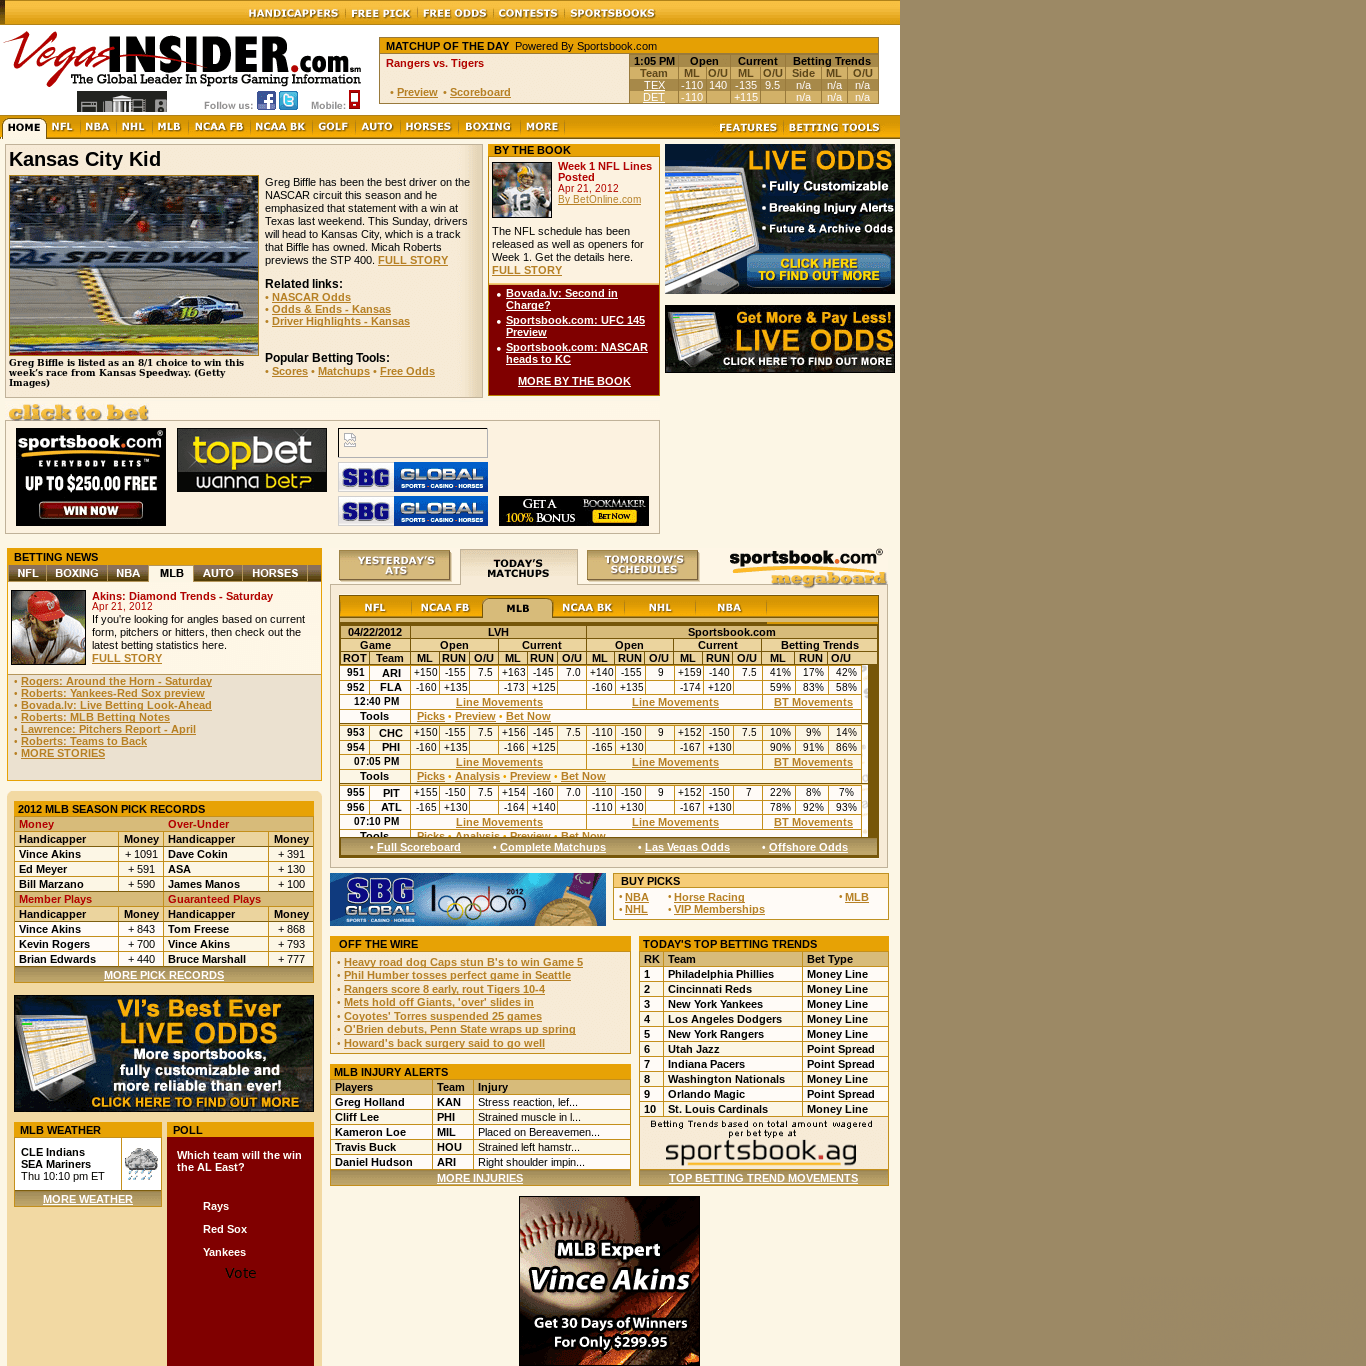
\includegraphics[width = 1in]{images/1-snapshot.png}} &
\subfloat{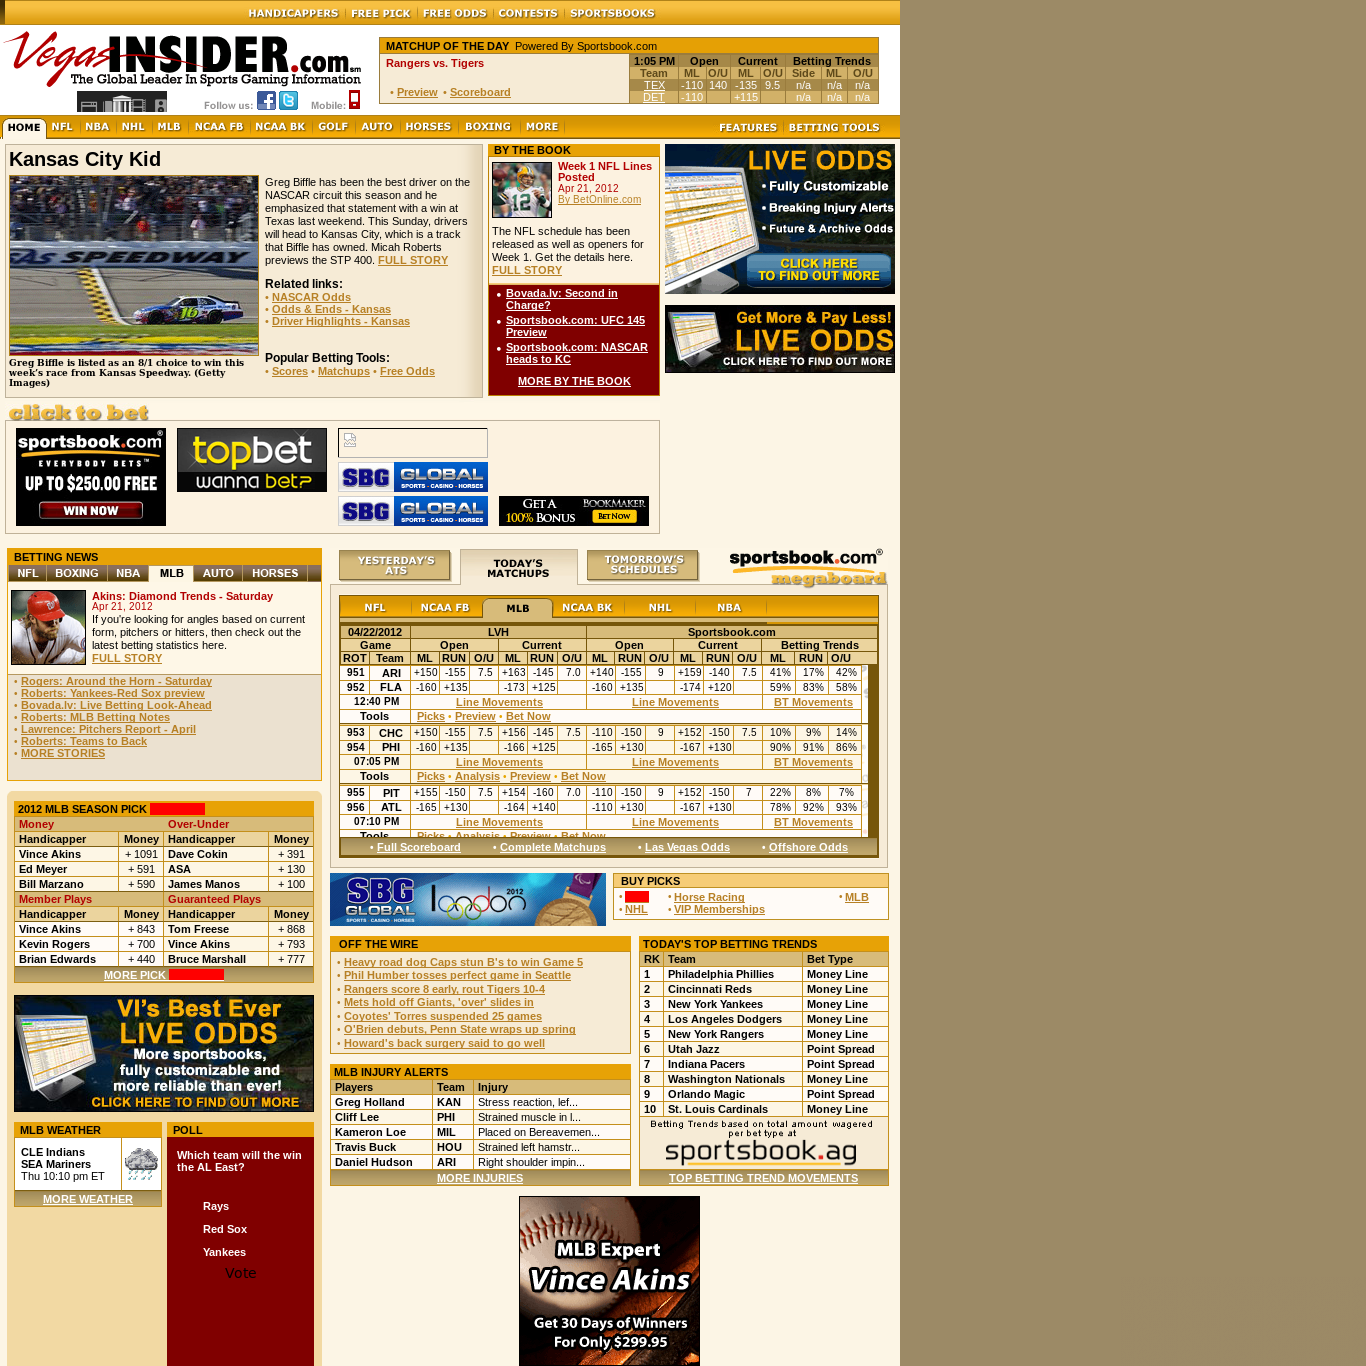
\includegraphics[width = 1in]{images/1-highlights.png}} &
\subfloat{
\includegraphics[width = 1in]{images/1-saliency.png}} \\
\subfloat{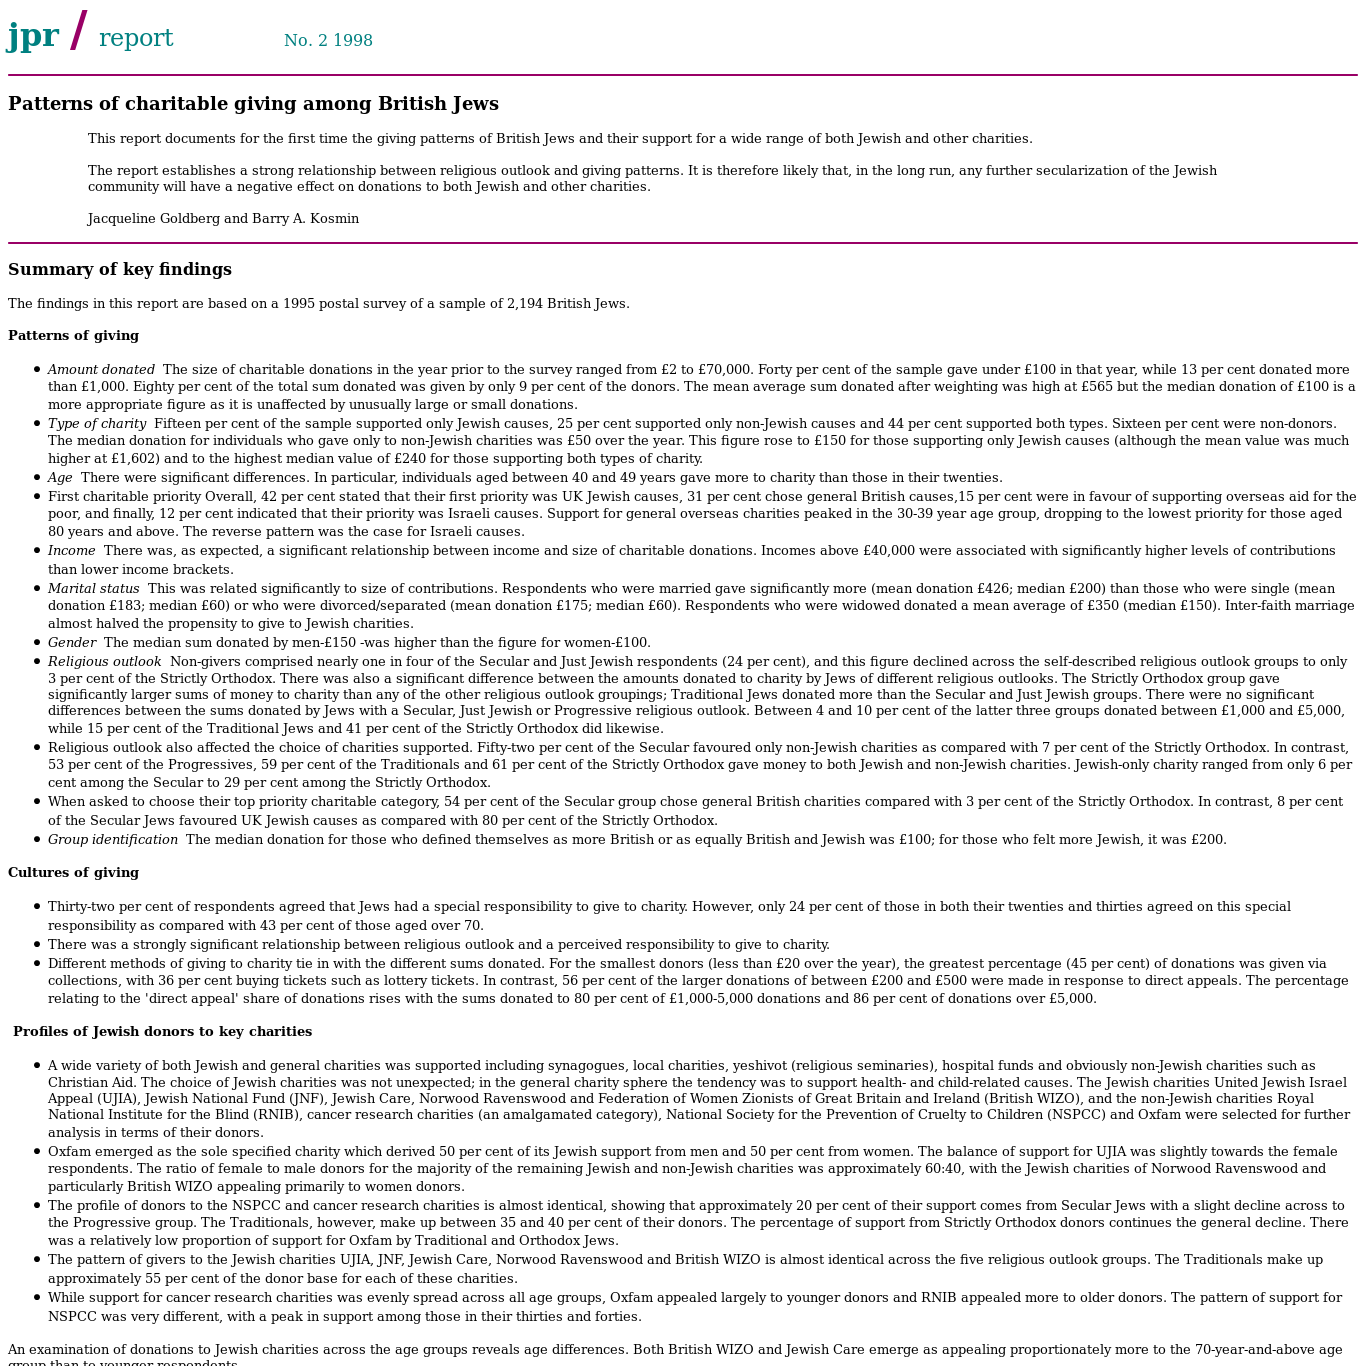
\includegraphics[width = 1in]{images/2-snapshot.png}} &
\subfloat{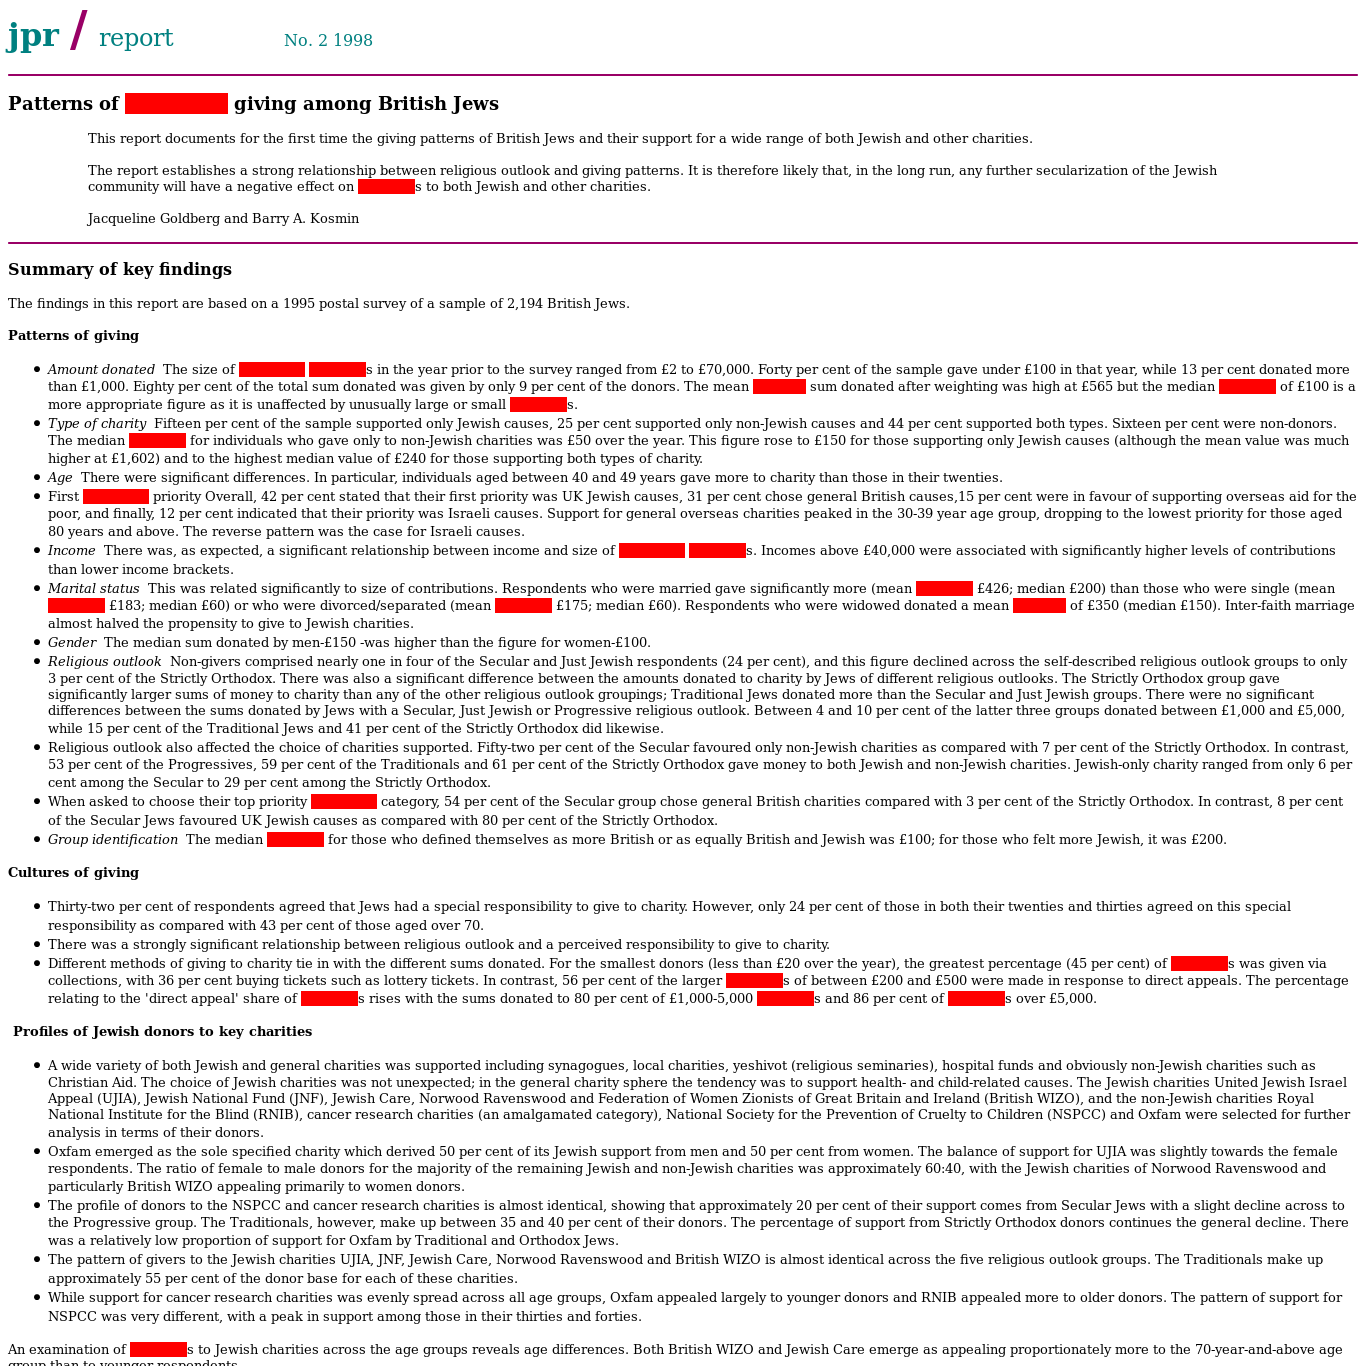
\includegraphics[width = 1in]{images/2-highlights.png}} &
\subfloat{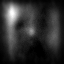
\includegraphics[width = 1in]{images/2-saliency.png}} \\
\subfloat{
\includegraphics[width = 1in]{images/3-snapshot.png}} &
\subfloat{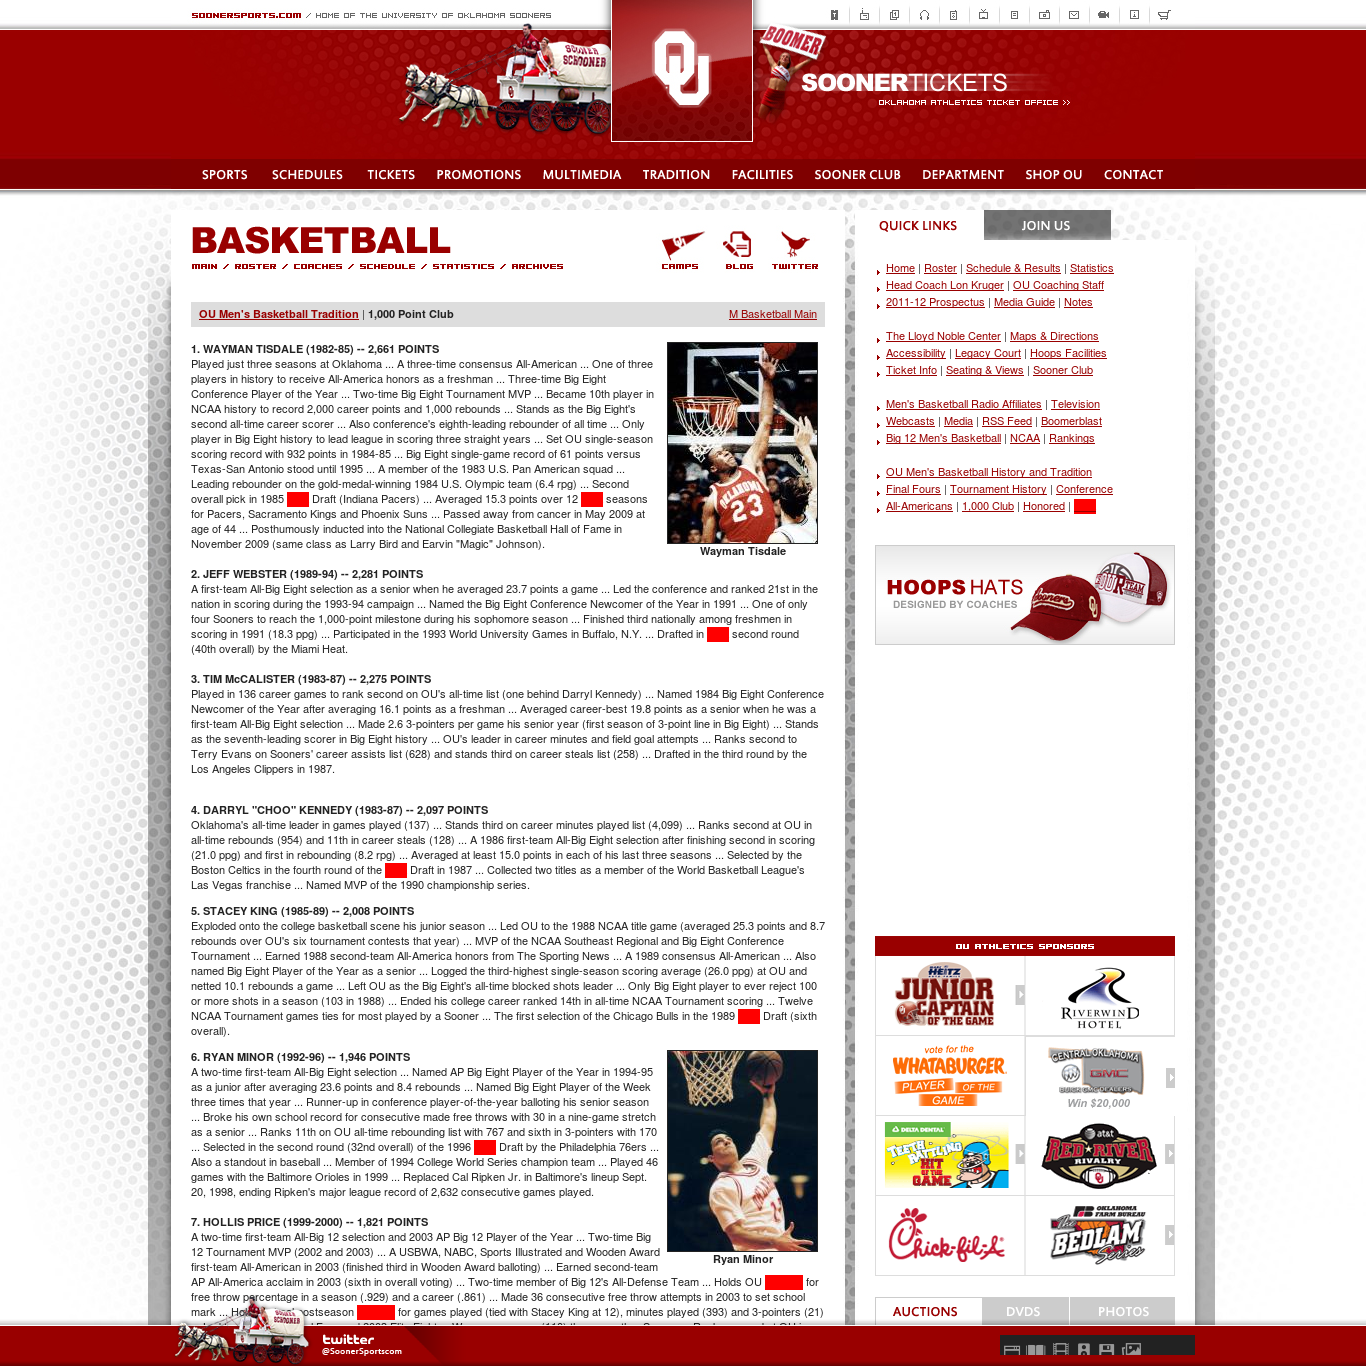
\includegraphics[width = 1in]{images/3-highlights.png}} &
\subfloat{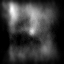
\includegraphics[width = 1in]{images/3-saliency.png}} \\
\end{tabular}
\caption{Examples of the vanilla snapshot, red highlighted snapshot and saliency heatmap from left to right respectively}\label{fig:exampleshots}
\end{figure}


\subsubsection{Filtering}\label{sec:datasetsum}
As the Wayback Machine does not contain an archived or working version of each document in the ClueWeb12 collection, a filtering process was introduced to maximize the quality of each snapshot. Using the following criteria, a snapshot was selected for each available document. 
\todo{@Maarten: could you compress this enumeration please?}
\begin{enumerate}    
\item Each document is requested from the Wayback Machine. 
\item A document that is not on the Wayback Machine, times out, throws a JavaScript error or results in a PNG snapshot smaller than 100KB is marked as broken. Such documents are rendered again using the online rendering service provided by ClueWeb12.
\item A manual selection is made between all documents that are rendered from both sources. The Wayback version is used if it contains more styling elements and if the content is the same as in the rendering service. Otherwise, the rendering service version is used. 
\end{enumerate}
%
At the end of the above process, most of 28,906 judged documents had a corresponding snapshot from either the Wayback Machine or ClueWeb12 rendering service.
Only 265 documents did not pass the filtering and were discarded.
The first row of Table \ref{tab:countsources} summarizes the results of the \datasetname~acquisition process.


\subsection{Content features} \label{sec:contentfeature}
In LTR, documents are ranked based on various content features, such as BM25 and PageRank.
We compute these content features by doing a full pass over the complete ClueWeb12 using Apache Spark.\footnote{This took us approximately 20 hours on 116 Hadoop worker nodes with 3 executor cores and 21gb memory each.}
During this process an HTML parser (jsoup\footnote{\url{https://jsoup.org/}} in our case) extracts the title and content from the raw HTML.
Because the HTML structure in very large documents cannot be parsed efficiently by jsoup, all documents with more than one million tokens are ignored.
Using the Apache Spark implementation of TF and IDF, a sparse vector is obtained for each term in each document. Finally, the sparse vectors are loaded into a Python Pandas dataframe, which is used to compute the TF, IDF, TFIDF and BM25 scores for each documents-query pair.

Additionally, PageRank scores from the ClueWeb12 Related Data section\footnote{\url{https://lemurproject.org/clueweb12/related-data.php}} are added to each document.
In total, 11 features are computed, summarized in Table \ref{tab:setdescription}.

Finally, the following modifications based on the features from LETOR 3.0~\cite{qin2010letor} are made to stabilize training:
\todo{@Maarten: could you also compress this one please?}
\begin{enumerate}  
% \item IDF is calculates as follows: 
% $$IDF(q, D) = \sum_{t_i \in q} IDF(t_i, D) = \sum_{t_i \in t} \log \frac{|D| + 1}{DF(t_i) + 1}$$
% Where  $q_i$ and $t_i$ represent a list of all terms in a query and a single query term respectively. $D$ represents a list of all terms in a document with $|D|$ as its total length. $DF(t_i)$ is the document frequency for the given query term.  
\item Free parameters $k_1$, $k_3$ and $b$ for BM25 were set to $2.5$, $0$ and $0.8$ respectively. 
\item Because the PageRank scores are usually an order of magnitude smaller than all the other scores, we multiply each value by $10^5$.
\item After all features are computed, the log is taken over the final results.
\item The logged features are normalized per query.  
\end{enumerate}

\begin{table}[h]
\centering
\captionof{table}{Content features provided with \datasetname.}  \label{tab:setdescription} 
\begin{tabular}{rlrlrl}
\toprule
Id & Description & Id & Description & Id & Description    \\ 
\midrule
1  & Pagerank  & 5  & Content TFIDF  & 9  & Title IDF   \\
2  & Content length & 6  & Content BM25   & 10 & Title TFIDF   \\
3  & Content TF  & 7  & Title length & 11 & Title BM25  \\
4  & Content IDF & 8  & Title TF  & & \\
\bottomrule
\end{tabular}
\end{table}



%\textit{(This has not been done yet)} The TF and IDF scores were also calculated Anchor text extracted by \citet{hiemstra2010mapreduce} 
% Make a seperate section for snapshots and subsections for collection, cleaning, statistics etc.


\subsection{Final collection}\label{sec:finalcollection}
In summary, \datasetname~contains:
\begin{inparaenum}[(i)]
\item a directory with web page snapshots (Section~\ref{sec:screenshotsec}), and
\item a set of files with content features divided into folds. (Section~\ref{sec:contentfeature}).
\end{inparaenum}
%\todo{Why do we have a set of files with features and not only one file?}


Each snapshot is stored as a PNG file which can be identified by its corresponding ClueWeb12 document id. 
The content features are stored in LETOR formatted files containing the raw, logged and query normalized values.
The query normalized values are randomly split per query into five equal fold-partitions.
These fold-partitions are then divided in five folds where each fold contains three fold-partitions for training and the remaining two for validation and testing.

%A separate file contains an entry for each snapshot indicating whether the snapshots was created using the Wayback Machine or online rendering service. 

%\begin{figure*}[t]
%\centering
%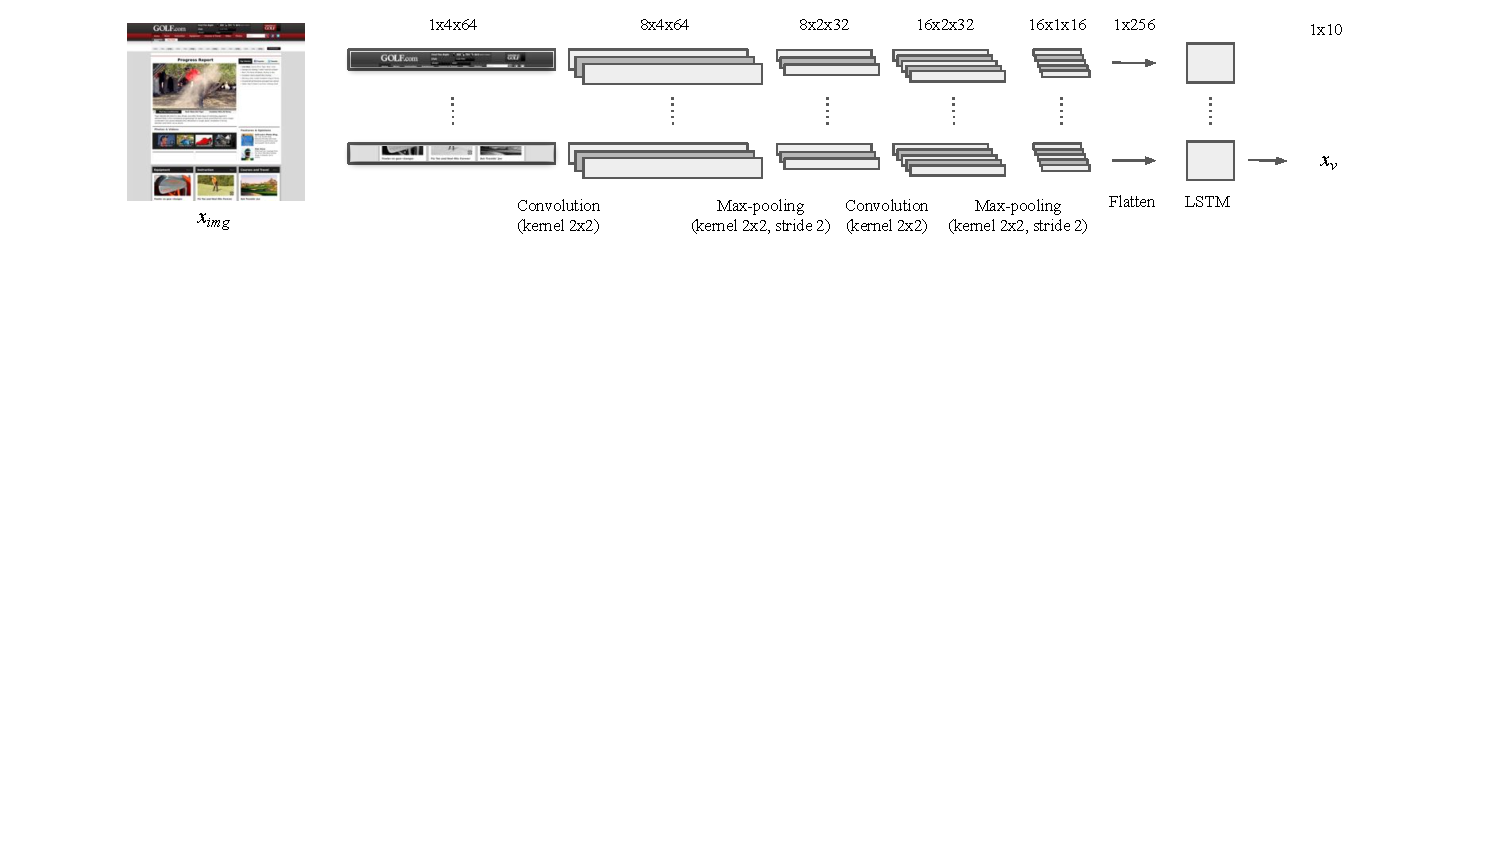
\includegraphics[clip,trim=0 10cm 0 0, width=20cm]{images/vip-features.pdf}
%  \captionof{figure}{The feature extractor architecture with corresponding dimensions used in our implementation of the ViP model.} \label{fig:ViPfeat} 
%\end{figure*}

% !TEX root = cikm2018-visual-ltr.tex

\section{The \protect\datasetname{} Data\-set}
In this section, we describe the \datasetname~data\-set. 
Section~\ref{sec:trecclue} contains information about the underlying ClueWeb12 collection and TREC Web Track topics. Section~\ref{sec:screenshotsec} explains how the snapshots for ClueWeb12 were acquired using the Wayback Machine\footnote{\url{http://archive.org/web/}} and ClueWeb12 Online rendering service.\footnote{\url{http://boston.lti.cs.cmu.edu/Services/}} Section~\ref{sec:contentfeature} discusses the details on how content features, such as BM25 and TF-IDF, are calculated using Apache Spark.\footnote{\url{https://spark.apache.org/}} Finally, Section~\ref{sec:finalcollection} gives an overview of the structure in which the \datasetname~dataset is presented.

\subsection{ClueWeb12 \& TREC Web Track}\label{sec:trecclue}
For \datasetname{} we choose to use a combination of the ClueWeb12 document collection and the topics from the TREC Web Tracks 2013 \& 2014~\cite{collins2013trec,collins2015trec},
because this is currently the most recent combination of a large-scale web page collection together with judged queries (with graded relevance). 

ClueWeb12 is a highly diverse collection of web pages scraped in the first half of 2012.
The total collection contains over 700 million documents that are crawled using the typical crawling settings of the Heritrix archival crawler project.\footnote{\url{https://webarchive.jira.com/wiki/spaces/Heritrix/overview}}

We only use ClueWeb12 documents that have been judged for any of the 100 queries in the TREC Web Tracks 2013 \& 2014. In total, there are 28,906 judged pages.

Table~\ref{tab:countsources} shows the breakdown of the total number of pages and different relevance labels in the combined set of topics from 2013 and 2014.

\begin{table}[h]
  \captionof{table}{The total number of documents per source and the corresponding breakdown of TREC Web Track relevance grades.} 
  \label{tab:countsources}
  \begin{tabular}{ l  @{}r  r  r  r }
  \toprule
    Count/Label & TREC Web & Wayback & ClueWeb12 & \mbox{}\hspace*{-.15cm}No image\\
    \midrule
    Total & 28,906 & 23,249 & 5,392 & 265 \\
    Nav grade (4) & 40 & 36 & 4 & 0\\
    Key grade (3) & 409 & 347 & 62 & 0\\
    Hrel grade (2) & 2,534 & 2,222 & 295 & 17 \\
    Rel grade (1) & 6,832 & 5,679 & 1,123 & 30\\
    Non grade (0) & 18,301 & 14,395 & 3,701 & 205 \\
    Junk grade (-2) & 790 & 570 & 207 & 13\\
    \bottomrule
  \end{tabular} 
\end{table}


\subsection{Snapshots} \label{sec:screenshotsec}
Although each entry in the ClueWeb12 collection contains the document's HTML source, many pages lack styling and images files in order to render the full page.
To overcome this issue, we use the Wayback Machine,\footnote{\url{http://archive.org/web/}} which offers various archived versions of web pages with styling and images since 2005.
For each page in CueWeb12 that is also judged in the TREC Web Tracks 2013 \& 2014 (see the first row in Table~\ref{tab:countsources})
we scrape an entry on the Wayback Machine that is closest to the original page scrape date as recorded in ClueWeb12.
A snapshot is then taken using a headless instance of the Firefox browser together with the Python implementation of the Selenium testing framework.\footnote{\url{http://selenium-python.readthedocs.io/}}
To reproduce \cite{fan2017learning}, we also create a separate query dependent dataset with the same snapshots where all query words are highlighted in red (HEX value: \#ff0000).
Examples of snapshots and snapshots with highlights are shown in Fig.~\ref{fig:exampleshots} (first two columns).

\begin{figure}[t]
\begin{tabular}{ccc}
\subfloat{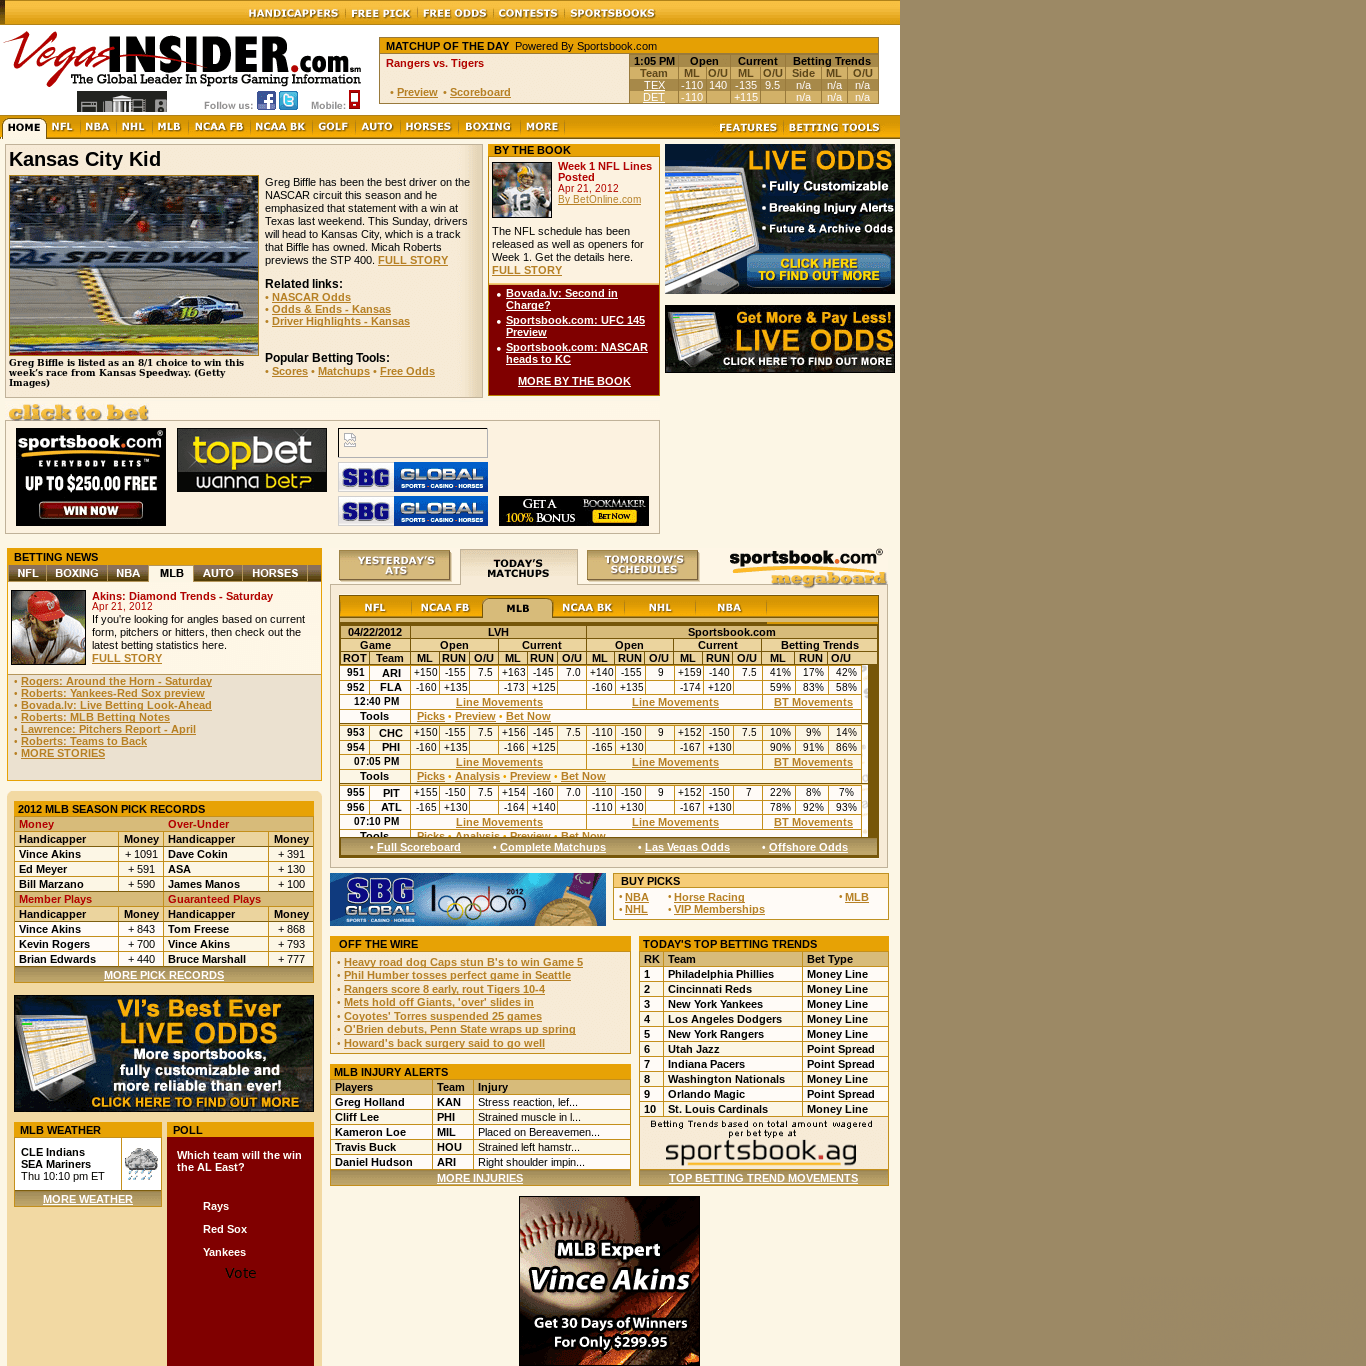
\includegraphics[width = 1in]{images/1-snapshot.png}} &
\subfloat{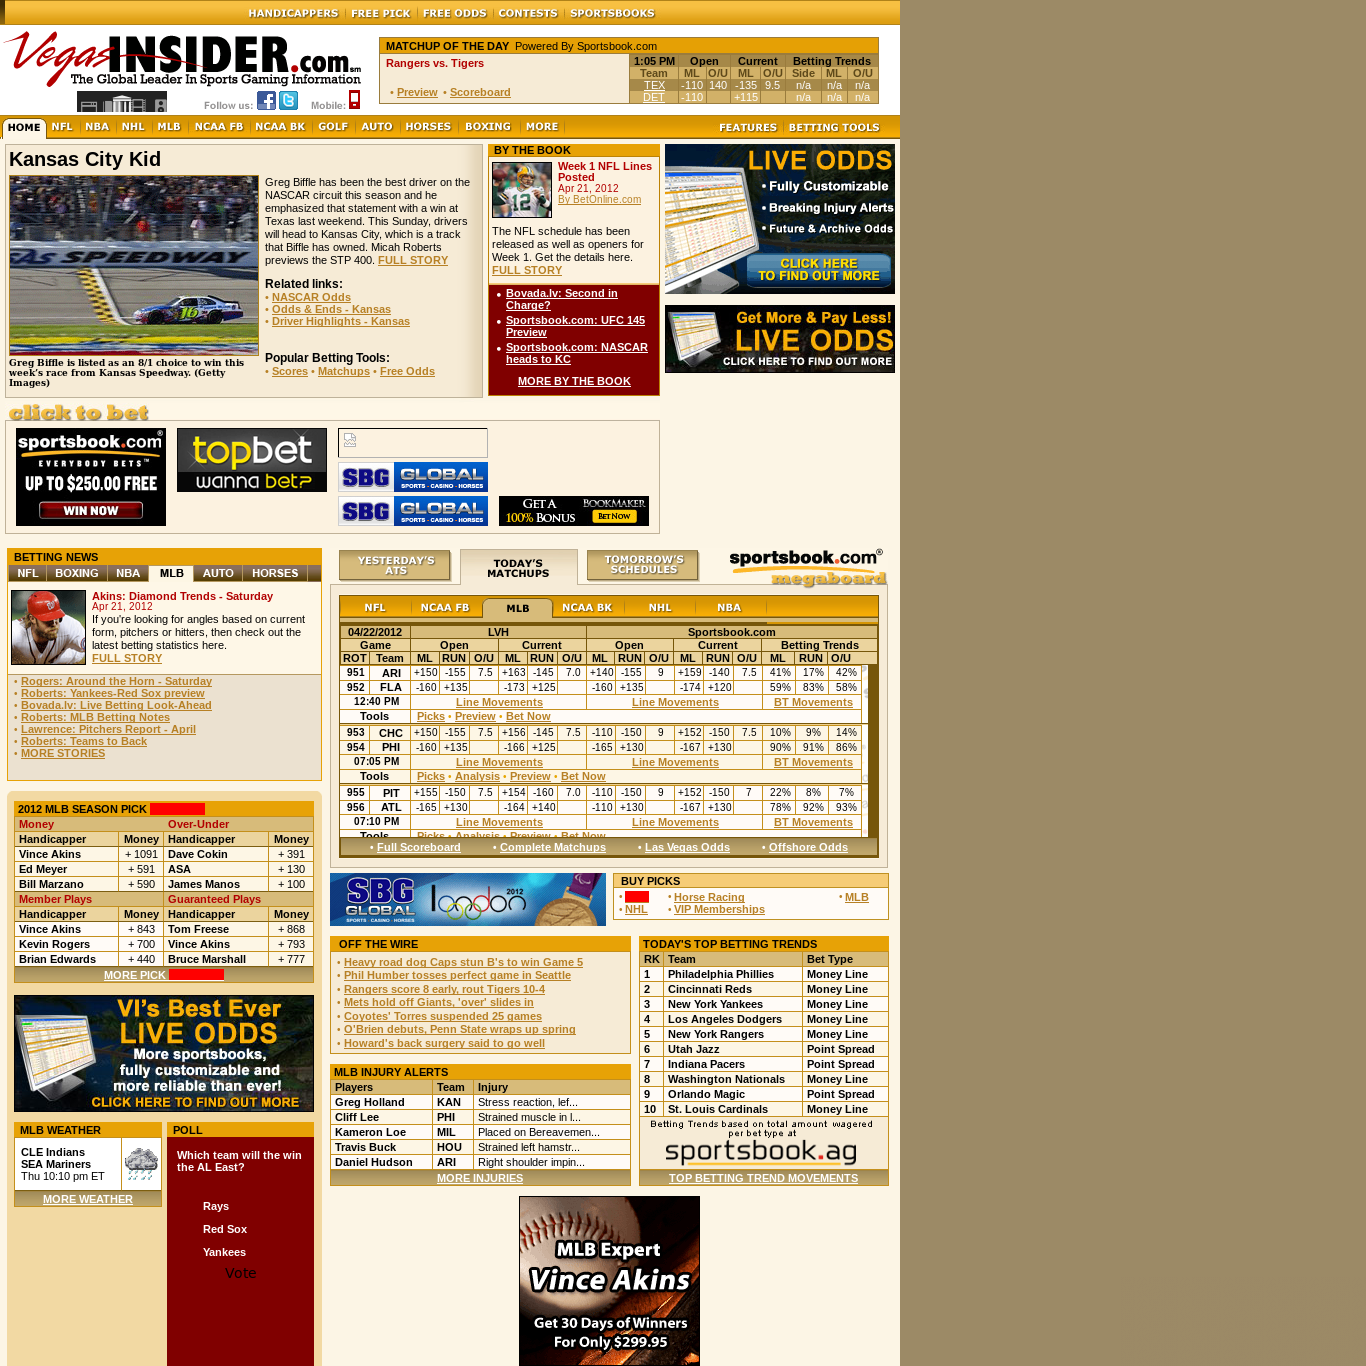
\includegraphics[width = 1in]{images/1-highlights.png}} &
\subfloat{
\includegraphics[width = 1in]{images/1-saliency.png}} \\
\subfloat{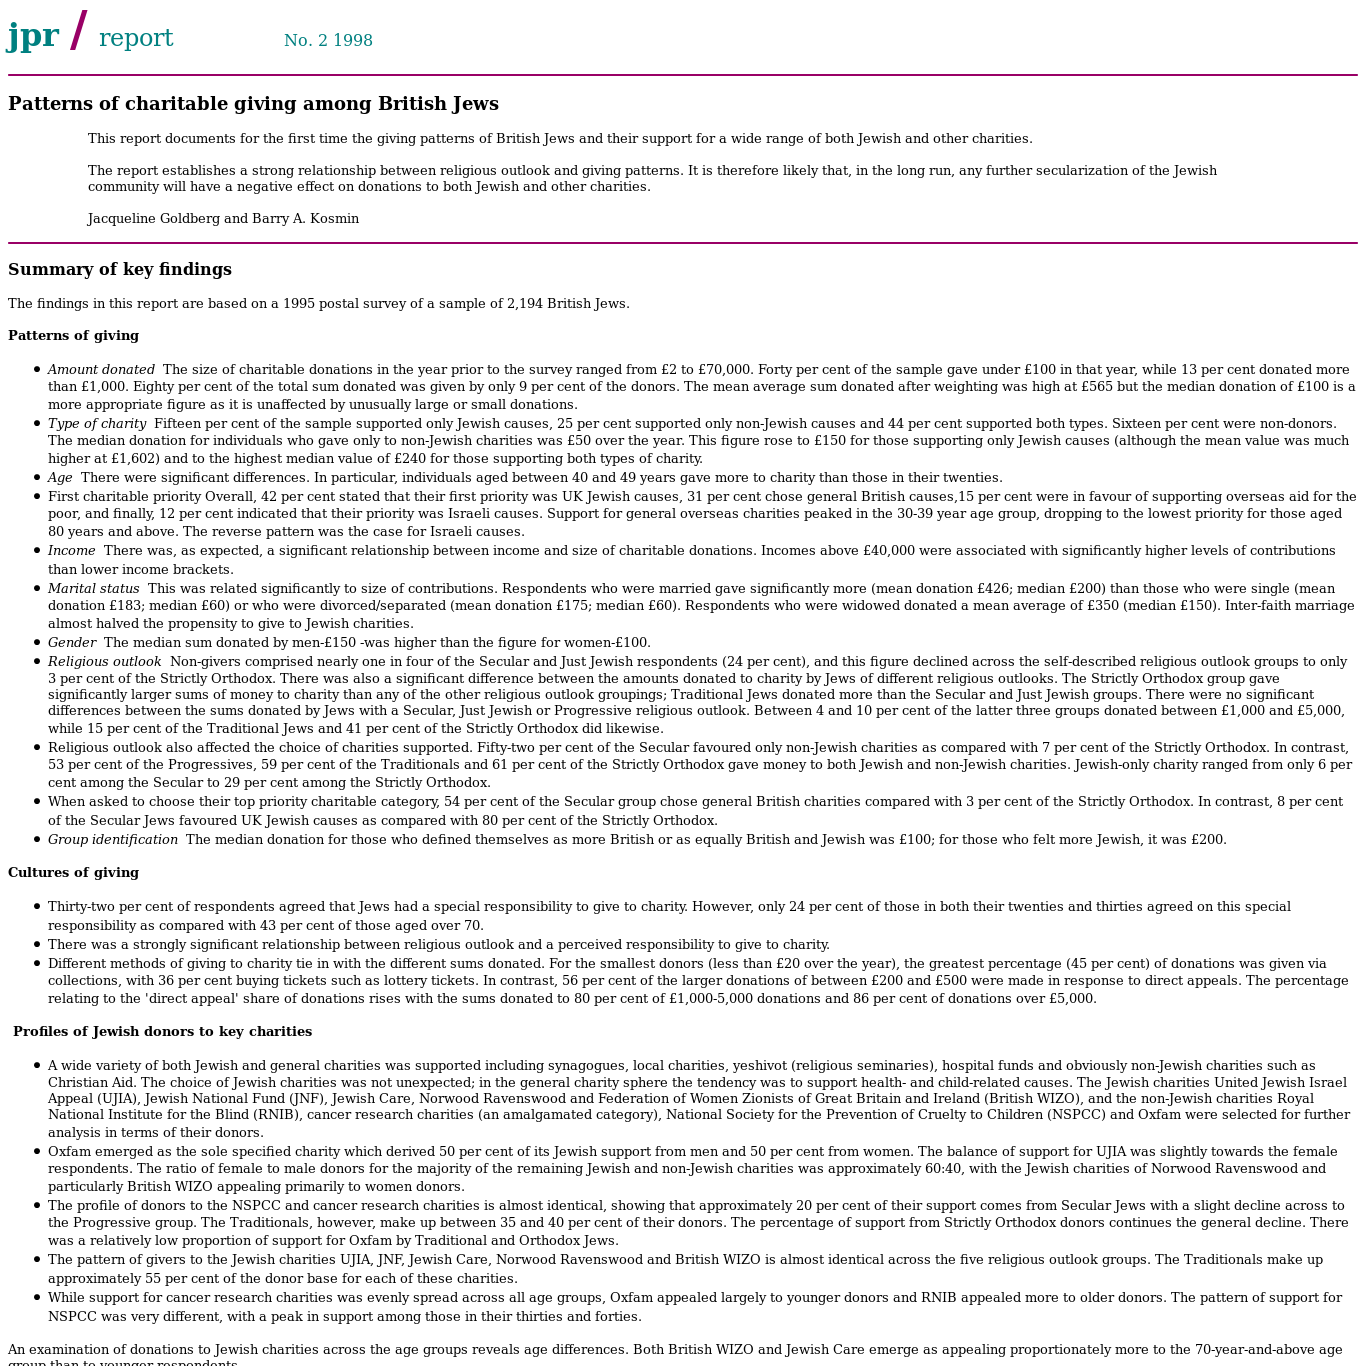
\includegraphics[width = 1in]{images/2-snapshot.png}} &
\subfloat{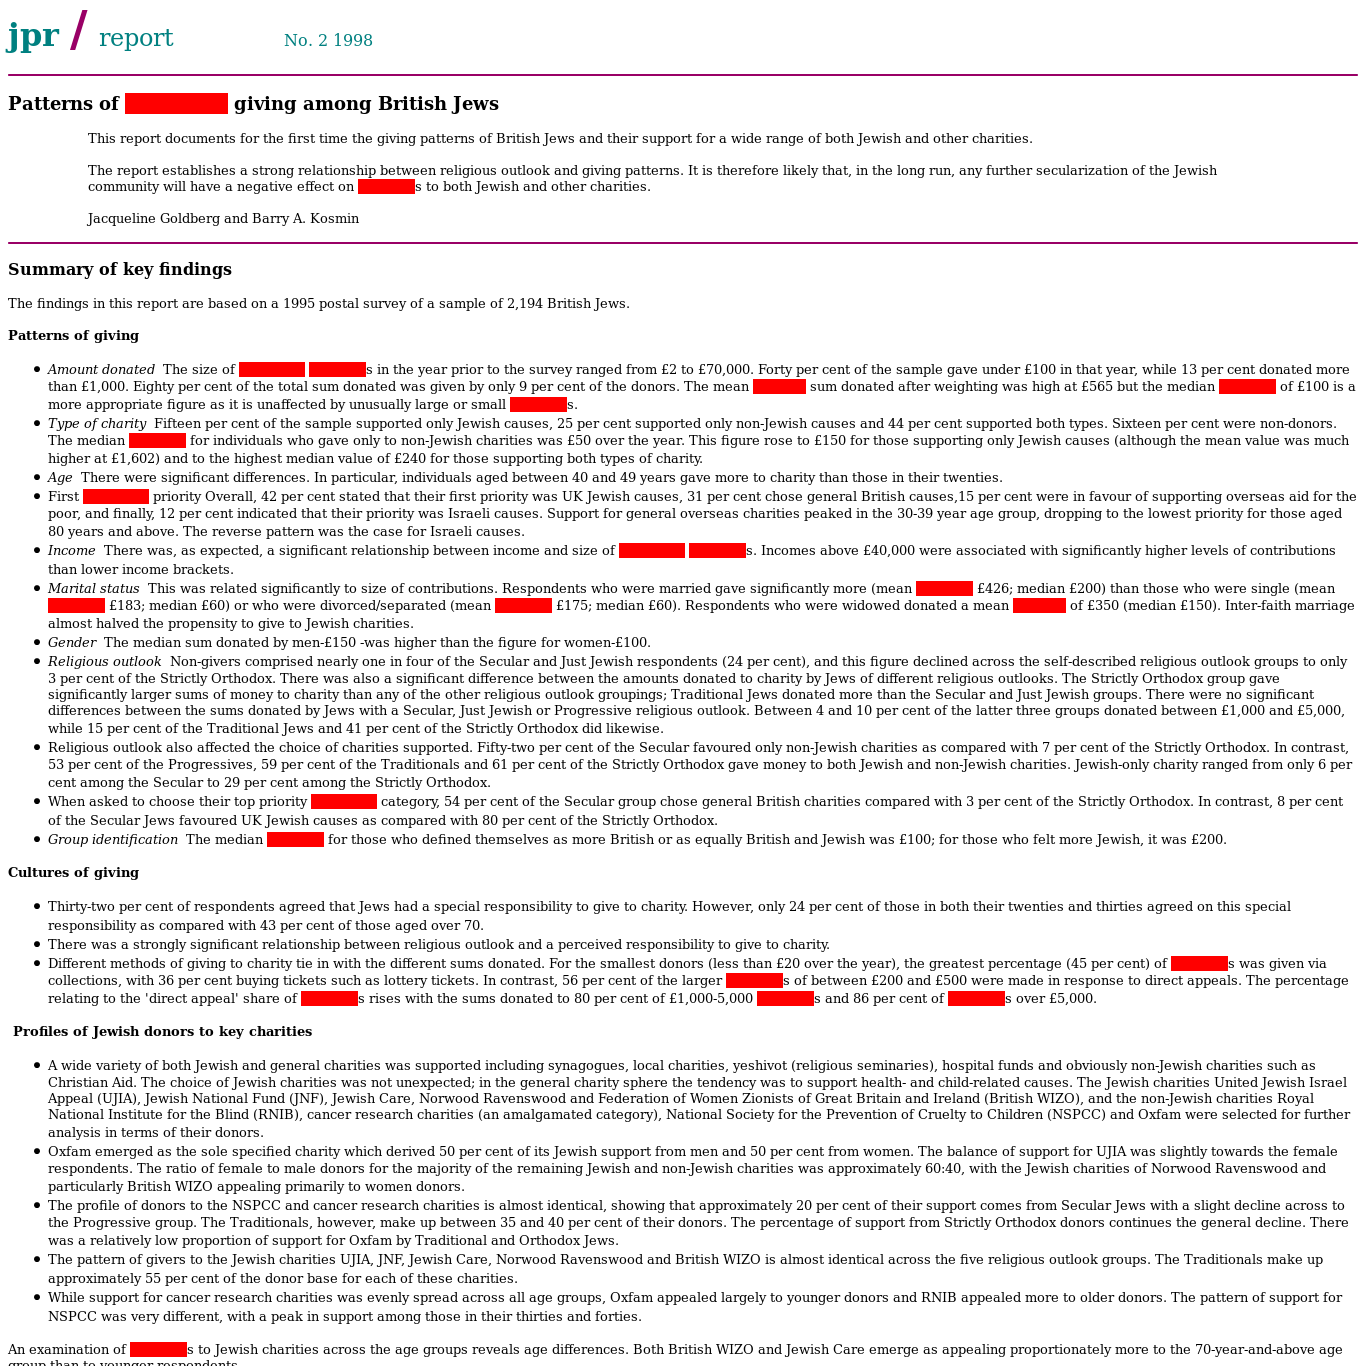
\includegraphics[width = 1in]{images/2-highlights.png}} &
\subfloat{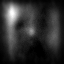
\includegraphics[width = 1in]{images/2-saliency.png}} \\
\subfloat{
\includegraphics[width = 1in]{images/3-snapshot.png}} &
\subfloat{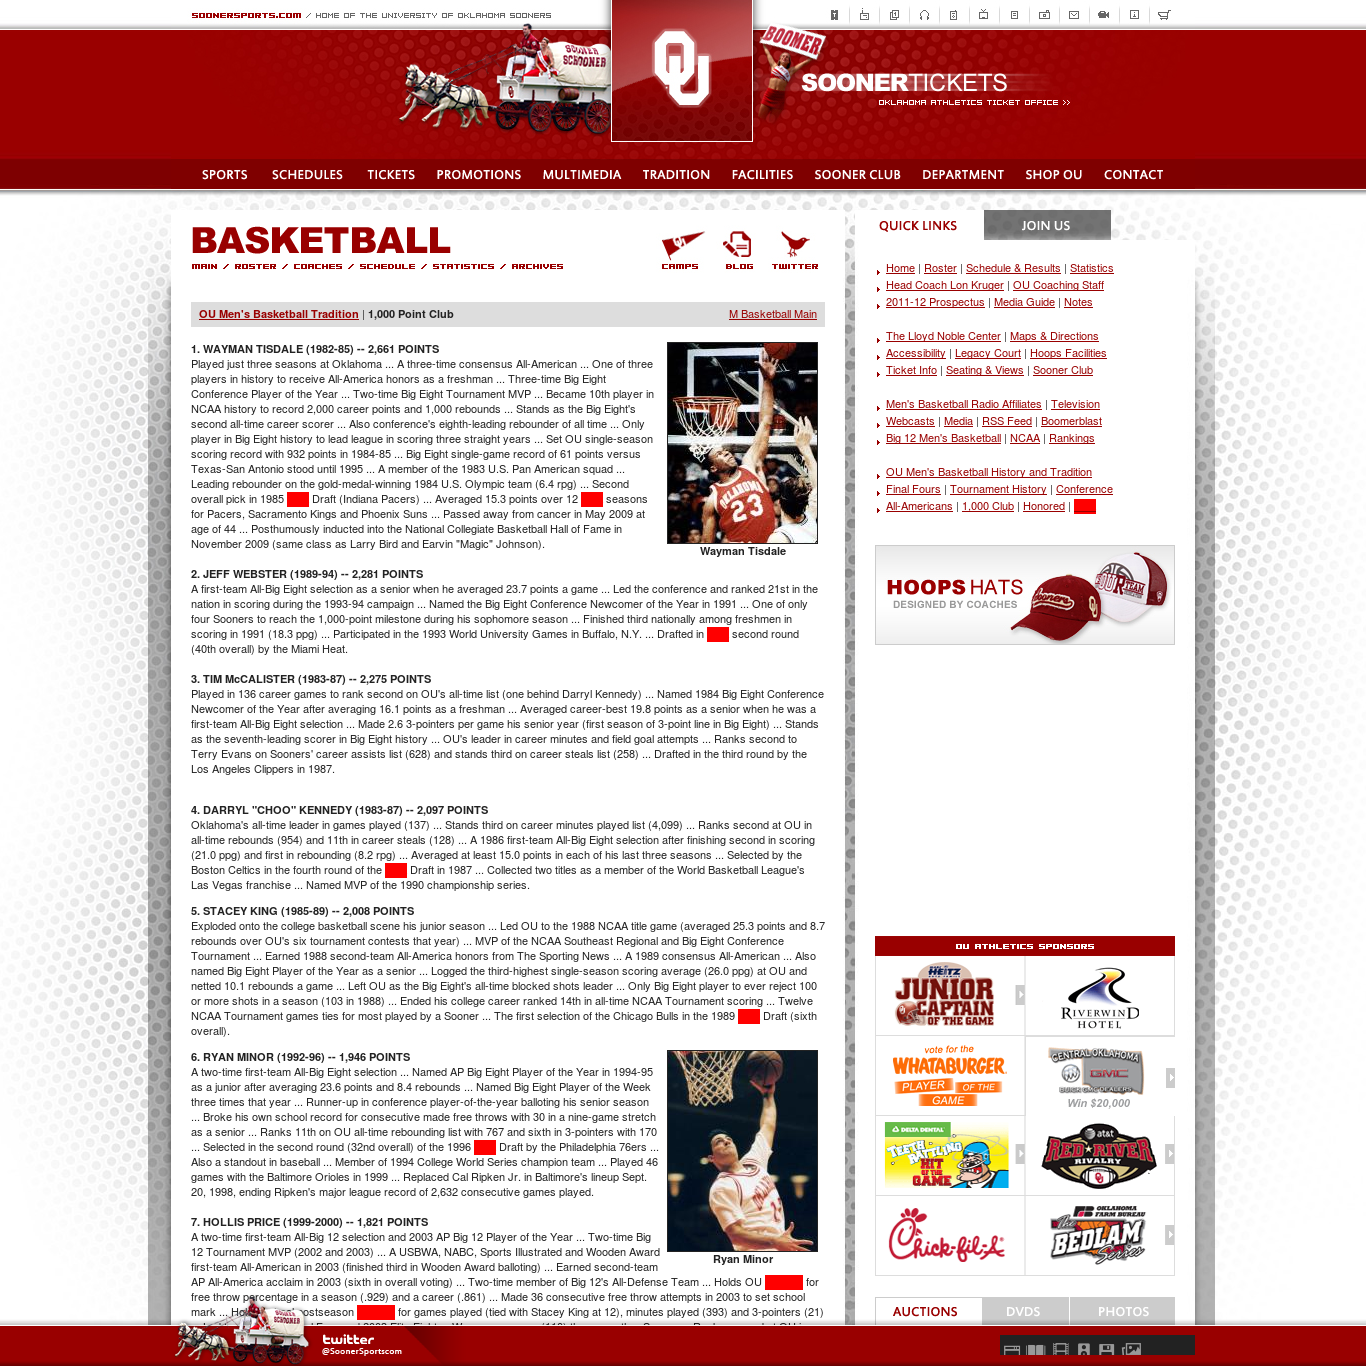
\includegraphics[width = 1in]{images/3-highlights.png}} &
\subfloat{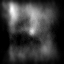
\includegraphics[width = 1in]{images/3-saliency.png}} \\
\end{tabular}
\caption{Examples of a vanilla snapshot, a red highlighted snapshot, and a saliency heatmap from left to right, respectively.}
\label{fig:exampleshots}
\end{figure}


\label{sec:datasetsum}
As the Wayback Machine does not contain an archived or working version of each document in the ClueWeb12 collection, a filtering process was introduced to maximize the quality of each snapshot. Using the following criteria, a snapshot was selected for each available document. 
\begin{enumerate}[nosep,leftmargin=14pt]
\item Each document is requested from the Wayback Machine. 
\item A document that is not on the Wayback Machine, times out, throws a JavaScript error or results in a PNG snapshot smaller than 100KB is marked as broken. Such documents are rendered again using the online rendering service provided by ClueWeb12.\footnote{\url{http://boston.lti.cs.cmu.edu/Services/}}
\item A manual selection is made between all documents that are rendered from both sources. The Wayback version is used if it contains more styling elements and if the content is the same as in the rendering service. Otherwise, the rendering service version is used. 
\end{enumerate}
%
As a result, most of the 28,906 judged documents had a corresponding snapshot from either the Wayback Machine or ClueWeb12 rendering service; only 265 documents did not pass the filtering and were discarded.
Table~\ref{tab:countsources}, row one, summarizes the results of the \datasetname~acquisition process.


\subsection{Non-Visual Features} 
\label{sec:contentfeature}
In LTR, documents are ranked based on various types of features, such as content features (BM25), quality indicators (PageRank) and behavioral features (CTR).
In order to use \datasetname~to measure the effect of visual features, we also add a set of content features and quality indicators.
In preliminary experiments, we compared the effect of reducing the 46 features in LETOR~\cite{qin2010letor} to just the 11 features described in Table~\ref{tab:setdescription}.
As these features are relatively easy to compute and the experiments showed a minimal drop in performance, we decided to limit ourselves to these features for \datasetname.
Also note that behavioral features, such as CTR, are not available for the TREC Web Tracks.

The content features are computed by doing a full pass over the complete ClueWeb12 collection using Apache Spark.\footnote{\url{https://spark.apache.org/}}$^{ }$\footnote{This took approximately 20 hours on 116 Hadoop worker nodes with 3 executor cores and 21Gb memory each.}
During this process an HTML parser (jsoup\footnote{\url{https://jsoup.org/}} in our case) extracts the title and content from the raw HTML.
Because the HTML structure in very large documents cannot be parsed efficiently by jsoup, all documents with more than one million tokens are ignored.
Using the Apache Spark implementation of TF and IDF, a sparse vector is obtained for each term in each document. Finally, the sparse vectors are loaded into a Python Pandas dataframe, which is used to compute the TF, IDF, TF-IDF and BM25 scores for each document-query pair.

Additionally, PageRank scores from the ClueWeb12 Related Data section\footnote{\url{https://lemurproject.org/clueweb12/related-data.php}} are added to each document.

Finally, the following modifications based on the feature transformations described in LETOR 3.0~\cite{qin2010letor} are made to stabilize training:
\begin{enumerate}[nosep,leftmargin=14pt]
% \item IDF is calculates as follows: 
% $$IDF(q, D) = \sum_{t_i \in q} IDF(t_i, D) = \sum_{t_i \in t} \log \frac{|D| + 1}{DF(t_i) + 1}$$
% Where  $q_i$ and $t_i$ represent a list of all terms in a query and a single query term respectively. $D$ represents a list of all terms in a document with $|D|$ as its total length. $DF(t_i)$ is the document frequency for the given query term.  
\item Free parameters $k_1$, $k_3$ and $b$ for BM25 were set to $2.5$, $0$ and $0.8$, respectively. 
\item Because the PageRank scores are usually an order of magnitude smaller than all other scores, we multiply each value by $10^5$.
\item After all features are computed, the log is taken over the final results.
\item The logged features are normalized per query.  
\end{enumerate}

\begin{table}[h]
\centering
\captionof{table}{Non-visual features provided with \datasetname.}  \label{tab:setdescription} 
\begin{tabular}{rlrlrl}
\toprule
Id & Description & Id & Description & Id & Description    \\ 
\midrule
1  & Pagerank  & 5  & Content TFIDF  & 9  & Title IDF   \\
2  & Content length & 6  & Content BM25   & 10 & Title TFIDF   \\
3  & Content TF  & 7  & Title length & 11 & Title BM25  \\
4  & Content IDF & 8  & Title TF  & & \\
\bottomrule
\end{tabular}
\end{table}

\subsection{Final Collection}\label{sec:finalcollection}
In summary, \datasetname~contains:
\begin{inparaenum}[(i)]
\item a directory with web page snapshots (Section~\ref{sec:screenshotsec}), and
\item a set of files with content features divided into folds (Section~\ref{sec:contentfeature}).
\end{inparaenum}
Each snapshot is stored as a PNG file that can be identified by its corresponding ClueWeb12 document id. 
The non-visual features are stored in LETOR formatted files containing the raw, logged and query normalized values.
The query normalized values are randomly split per query into five equal partitions.
These partitions are then used to create five folds, where each fold contains three partitions for training and the remaining two partitions for validation and testing.

%A separate file contains an entry for each snapshot indicating whether the snapshots was created using the Wayback Machine or online rendering service. 


% !TEX root = cikm2018-visual-ltr.tex

%\section{Experimental Setup}\label{sec:experiments}
%In this section, we discuss the setup of the experiments performed on \datasetname. The experiments are set out to demonstrate the abilities of visual features in LTR and set a baseline for future visual LTR research.
%%All PyTorch experiments were performed on a GTX 1080 Ti with 11gb of RAM. Preprocessing was performed on a Thinkpad X250 with an Intel i5-5300U CPU and 16gb of ram. 
%
%\paragraph{\ac{LTR} with visual features}
%To average out the difference caused by random initialization, the experiments on \ac{LTR} with visual features are run five times for each of the five folds. 
%Each run is performed using the Adam optimizer with a batch size of 100 using a learning rate of $0.0001$ and $0.00005$ for the ViP and VGG-16 models respectively. These values were found empirically to find the highest performance for each model.
%Within each fold, the results for all five runs are averaged to create one measurement per fold per query.

% !TEX root = cikm2018-visual-ltr.tex


\section{Experiments and Results}
In this section, we discuss experiments performed on the proposed \datasetname~dataset.
These experiments are set out to test whether:
\begin{inparaenum}[(i)]
\item the \modelname~model can improve the \ac{LTR} performance when introducing visual feature vectors. 
\item synthetic saliency heatmaps improve the \ac{LTR} performance when used as an input the \modelname model, and
\item the \modelname~model results can improve both visual and non-visual state-of-the-art \ac{LTR} methods.
\end{inparaenum}

\subsection{Experimental Setup}
The experiments are divided into two types of setups:
\begin{inparaenum}[(i)]
\item baseline experiments using only content features, and
\item visual experiments using both content and visual features.
\end{inparaenum}

The \modelname~baseline refers to the baseline that demonstrates the performance increase of introducing visual features. We do so by using the \modelname~model and feeding the content features into the scoring component directly, without adding any visual features. 
The other content baseline experiments are performed using BM25 and the RankLib\footnote{\url{https://sourceforge.net/p/lemur/wiki/RankLib/}} implementations of RankBoost, AdaRank, and LambdaMart.

As a baseline comparison for our multimodal model, we implement ViP, the visual feature extractor proposed in~\citet{fan2017learning} using PyTorch. We train ViP on both the vanilla and highlighted snapshot datasets with the results being referred to as ViP snapshots and ViP highlights respectively.

The performance of the \modelname~model is demonstrated by learning visual feature vectors using VGG-16 and ResNet-152. Similarly as with the ViP model, both VGG-16 and ResNet-152 are trained on both the vanilla and highlighted snapshot dataset. 

Finally, we use the synthetic saliency heatmaps as an input to the \modelname~model. For the saliency heatmaps, we again use both VGG-16 and ResNet-152 to learn the visual feature vectors.

Each run is generated using the Adam optimizer with a batch size of $100$. The learning rates for all ResNet-152 and VGG-16 setups were set to $0.00005$ and $0.0001$ respectively. We empirically found that these values yield the highest performance for each model.

To measure the retrieval performance, we used precision and ndcg at $\{1,10\}$ and MAP.
Significance is determined using a two-tailed paired t-test (p-value $\leq 0.05$). 

All PyTorch experiments were performed on a single GTX 1080 Ti GPU with 11gb of RAM. 
% Preprocessing was performed on a Thinkpad X250 with an Intel i5-5300U CPU and 16gb of ram. 


\subsection{Results}
In this section we will compare and discuss the results of the 
\begin{inparaenum}[(i)]
\item \modelname~implementions, 
\item non-visual baselines, and 
\item visual baselines.
\end{inparaenum}  

\paragraph{\modelname~model with VGG-16 and ResNet-152}
In Table~\ref{tab:letorvisresults}, we compare the performance of the \modelname~model when used with and without visual feature vectors. The first row shows the \modelname~baseline, when using only the content features as an input to the scoring component. The second to fifth rows shows the performance of using VGG-16 and ResNet-152 with both vanilla and highlighted snapshots. 
These results clearly show that each of the methods of learning visual feature vectors significantly improves the \ac{LTR} performance of the \modelname~model compared to the \modelname~baseline. 

When comparing the results of using visual feature vectors we observe the following:
\begin{inparaenum}[(i)]
\item the highest ranking performance is achieved by using VGG-16 on the highlighted snapshots, 
\item performance on all performance metrics is consistently better when comparing highlighted with vanilla snapshots using VGG-16, which is not the case when comparing the two datasets using ResNet-152, and 
\item the performance increase for p@1 and ndcg@1, with an average of $+0.200$ and $+0.118$, is consistently higher than p@10 and ndcg@10, with an average of $+0.134$ and $+0.087$.
\end{inparaenum}

\begin{table}[h]
\caption{The \ac{LTR} results for the \modelname~model using vanilla snapshots, highlighted snapshots, saliency heatmaps and content features only. All results have a significant improvement over the \modelname~baseline. }
\label{tab:letorvisresults}
\centering
\begin{tabular}{l\OK l\OK l\OK l\OK l\OK l}
\toprule
                      & p@1    & p@10  & ndcg@1  & ndcg@10 & MAP   \\ 
\midrule
\modelname~baseline & 0.338  & 0.370 & 0.189   & 0.233   & 0.415 \\ 
\midrule
VGG snapshots      & 0.514 & 0.484 & 0.292 & 0.324 & 0.442 \\ 
ResNet snapshots   & 0.550 & 0.452 & 0.310 & 0.301 & 0.437 \\ 
VGG highlights     & \textbf{0.560} & \textbf{0.520} & 0.323 & \textbf{0.346} & \textbf{0.456} \\ 
ResNet highlights  & 0.530 & 0.463 & 0.305 & 0.312 & 0.440 \\
\midrule
VGG saliency       & 0.554 & 0.453 & 0.310   & 0.302   & 0.422 \\ 
ResNet saliency    & \textbf{0.560} & 0.476 & \textbf{0.333} & 0.321 & 0.442 \\
\bottomrule
\end{tabular}
\end{table}

\paragraph{\modelname~model with synthetic saliency heatmaps}
The last two rows of Table~\ref{tab:letorvisresults} shows the \ac{LTR} performance when using synthetic saliency heatmaps as an input to the \modelname~model. Similarly as the vanilla and higlighted snapshots, the visual feature vectors are learned by using both VGG-16 and ResNet-152. In contract to the vanilla and highlighted snapshots, ResNet-152 seems to consistently outperform VGG-16 when using synthetic saliency images. Although the highlighted snapshots with VGG-16 still outperform ResNet-152 with synthetic saliency images on p@10, ndcg@10 and MAP, the synthetic saliency images match and outperform performance when looking at p@1 and ndcg@1, respectively. 

\paragraph{Baseline comparison}
Table~\ref{tab:baseresults} compares the performance of the \modelname~model compared to both BM25, non-visual \ac{LTR} methods and the ViP model by~\citet{fan2017learning}. 
The table also shows both VGG-16 with highlighted snapshots and ResNet-152 with synthetic saliency heatmaps. Because these two results yield the highest \ac{LTR} performance, they are used to compare the \modelname~model with the baselines. 
We clearly see that both methods have a significant performance increase compared to using BM25, almost doubling the \ac{LTR} metrics.
Although both \modelname~implementations seem to consistently outperform all non-visual \ac{LTR} methods, we cannot confirm the statistical significance of each of the performance measures. 
However, we do find a significant improvement by the \modelname~implementations on the AdaRank \ac{LTR} results. Furthermore, when using VGG-16 with highlighted snapshots there is a significant performance increase in ndcg@10 compared to LambdaMart and in p@10 for both RankBoost and LambdaMart.

Finally, we compare the results of the \modelname~implementations with ViP as a visual \ac{LTR} baseline. 
Here we clearly see that both our implementations significantly outperform ViP on all measures. 

\paragraph{ViP results on \datasetname}
As addressed in the introduction, both the ViP model and the dataset used by~\citet{fan2017learning} have a number of limitations. The results in Table~\ref{tab:baseresults} clearly show that the limitations in the ViP model become apparent when being used with the more diverse and rich \datasetname~dataset. We do see that the results show a similar pattern as described by ~\citet{fan2017learning} where the model performs better when using highlighted snapshots compared to vanilla snapshots. However, using ViP with vanilla and highlighted snapshots from the \datasetname~dataset is outperformed by both RankBoost and LambdaMart. 

\begin{table}[h]
\caption{The $\dagger$ indicates a significant decrease in performance compared to the VGG-16 model with highlighted snapshots and $\ddagger$ indicates a significant decrease in performance for both \modelname~model results.}

\label{tab:baseresults}
\begin{tabular}{l\OK l\OK l\OK l\OK l\OK l}
\toprule
                      & p@1    & p@10  & ndcg@1  & ndcg@10 & MAP   \\
\midrule
BM25                  & 0.300$^\ddagger$  & 0.316$^\ddagger$ & 0.153$^\ddagger$   & 0.188$^\ddagger$   & 0.350$^\ddagger$ \\ 
\midrule
RankBoost             & 0.450  & 0.444 & 0.258   & 0.288$^\dagger$    & 0.427 \\
AdaRank               & 0.290$^\ddagger$   & 0.357$^\ddagger$  & 0.149$^\ddagger$    & 0.227$^\ddagger$    & 0.398 \\
LambdaMart            & 0.470  & 0.420$^\dagger$ & 0.256   & 0.275$^\dagger$    & 0.418 \\ 
\midrule
ViP snapshots         & 0.392$^\ddagger$ & 0.398$^\ddagger$ & 0.217$^\ddagger$   & 0.254$^\ddagger$   & 0.421$^\ddagger$ \\ 
ViP highlights        & 0.418$^\ddagger$  & 0.416$^\ddagger$ & 0.239$^\ddagger$   & 0.269$^\ddagger$   & 0.422$^\ddagger$ \\
\midrule
VGG highlights        & \textbf{0.560}  & \textbf{0.520} & 0.323   & \textbf{0.346}   & \textbf{0.456} \\ 
ResNet saliency       & \textbf{0.560} & 0.476 & \textbf{0.333} & 0.321 & 0.442 \\
\bottomrule
\end{tabular}
\end{table}




% !TEX root = www2019-visual-ltr.tex

\section{Results}
\label{sec:results}
%In this section, we present experiments that are set out to test the following:
%\begin{inparaenum}[(1)]
%    \item the \modelname~model improves the \ac{LTR} performance when introducing visual features, 
%    \item synthetic saliency heatmaps improve the \ac{LTR} performance when used as an input the \modelname{} model, and
%    \item the \modelname~model improves both visual and non-visual state-of-the-art ranking methods.
%%    \item the results of the baseline ViP model~\cite{fan2017learning} are reproduced on the \datasetname{} dataset.
%\end{inparaenum}

\subsection{\modelname~model with VGG-16 and ResNet-152}
In Table~\ref{tab:letorvisresults}, we compare the performance of the \modelname~model when used with and without visual features.
The first row shows the \modelname~baseline, when using only the content features as an input to the scoring component.
The second to fifth rows show the performance of using VGG-16 and ResNet-152 with both vanilla and highlighted snapshots. 
These results clearly show that both VGG-16 and ResNet-152 visual feature extraction methods significantly improve the performance compared to the \modelname~baseline. 

When comparing the results of the \modelname~model with visual features, we observe the following:
\begin{inparaenum}[(i)]
    \item The highest ranking performance is achieved by using VGG-16 on the highlighted snapshots.
    \item For VGG-16, the values of all metrics are consistently better for highlighted snapshots compared to vanilla snapshots, which is in line with the findings of~\cite{fan2017learning} and is to be expected: highlighted snapshots carry more information compared to vanilla snapshots.
\end{inparaenum}
Based on these results, we conclude that the use of visual features in \ac{LTR} significantly improves performance
and that highlighted snapshots should on average be preferred over vanilla snapshots.
%These results are in line with the findings of~\cite{fan2017learning}.

\begin{table}[t]
\caption{Results for the \modelname~model using only content features (baseline), vanilla snapshots, highlighted snapshots, and saliency heatmaps.
All results significantly improve over the \modelname~baseline.
Best results are shown in bold.}
\label{tab:letorvisresults}
\centering
\begin{tabular}{l\OK l\OK l\OK l\OK l\OK l}
\toprule
                      & p@1    & p@10  & ndcg@1  & ndcg@10 & MAP   \\ 
\midrule
\modelname~baseline & 0.338  & 0.370 & 0.189   & 0.233   & 0.415 \\ 
\midrule
VGG snapshots      & 0.514 & 0.484 & 0.292 & 0.324 & 0.442 \\ 
ResNet snapshots   & 0.550 & 0.452 & 0.310 & 0.301 & 0.437 \\ 
VGG highlights     & \textbf{0.560} & \textbf{0.520} & 0.323 & \textbf{0.346} & \textbf{0.456} \\ 
ResNet highlights  & 0.530 & 0.463 & 0.305 & 0.312 & 0.440 \\
\midrule
VGG saliency       & 0.554 & 0.453 & 0.310   & 0.302   & 0.422 \\ 
ResNet saliency    & \textbf{0.560} & 0.476 & \textbf{0.333} & 0.321 & 0.442 \\
\bottomrule
\end{tabular}
\vspace*{-.5\baselineskip}
\end{table}


\subsection{\modelname{} model with saliency heat maps}
The last two rows of Table~\ref{tab:letorvisresults} show the performance of the \modelname{} mo\-del when using synthetic saliency heat maps as an input.
The visual features are learned using both VGG-16 and ResNet-152.
In this case, ResNet-152 consistently outperforms VGG-16.
Although the highlighted snapshots with VGG-16 still outperform ResNet-152 with saliency heat maps on p@10, ndcg@10 and MAP, the saliency heat maps with ResNet-152 match and outperform VGG-16 with highlighted snapshots when looking at p@1 and ndcg@1. 
Hence, saliency heat maps should be preferred in applications where early precision is important,
while highlighted snapshots should be used when a high overall performance is needed. 
%However, it is yet unclear what causes these differences,


\subsection{Baseline comparison}
Table~\ref{tab:baseresults} compares the performance of the \modelname~model to BM25, non-visual \ac{LTR} methods and the ViP model by~\citet{fan2017learning}. 
The table shows the performance of VGG-16 with highlighted snapshots and of ResNet-152 with synthetic saliency heatmaps, as these are the best-performing variants of the \modelname~model according to Table~\ref{tab:letorvisresults}.
%Because these two results yield the highest \ac{LTR} performance, they are used to compare the \modelname~model with the baselines. 
Both methods have a significant performance increase compared to BM25, almost doubling the metrics values in many cases.

When comparing to non-visual \ac{LTR} methods, both \modelname~implementations show consistently better performance.
However, not all metrics are improved significantly.
%However, we do find a significant improvement by the \modelname~implementations on the AdaRank \ac{LTR} results.
%Furthermore, when using VGG-16 with highlighted snapshots there is a significant performance increase in ndcg@10 compared to LambdaMart and in p@10 for both RankBoost and LambdaMart.
We attribute this to the fact that, similarly to~\cite{fan2017learning}, the \ac{LTR} component of the \modelname{} model is based on pairwise hinge loss, which is a relatively simple loss function.
%As a future work, we plan to investigate the effect of different loss functions on the performance of the \modelname{} model.

Finally, we compare the \modelname~implementations to ViP, the only existing \ac{LTR} method with visual features.
Here, we clearly see that both our implementations significantly outperform ViP on all metrics.
Also note, that ViP loses to two out of three non-visual \ac{LTR} baselines, namely RankBoost and LambdaMart.
We believe this is due to the reason discussed above: ViP uses pairwise hinge loss as the \ac{LTR} component~\cite{fan2017learning}, which may be suboptimal.

The above results show that the proposed \modelname{} model outperforms baselines, whether they are supervised or unsupervised, use visual features or not.
However, to achieve consistent significant improvements compared to the state-of-the-art \ac{LTR} methods, different loss functions within the \modelname{} model have to be investigated.


\begin{table}[t]
\caption{Results for the VGG-16 with highlighted snapshots, ResNet-152 with saliency heatmaps, and baselines.
$\dagger$ indicates a significant decrease in performance compared to VGG highlights and $\ddagger$ indicates a significant decrease in performance compared to both \modelname{} implementations.
Best results are shown in bold.}

\label{tab:baseresults}
\begin{tabular}{l\OK l\OK l\OK l\OK l\OK l}
\toprule
                      & p@1    & p@10  & ndcg@1  & ndcg@10 & MAP   \\
\midrule
BM25                  & 0.300$^\ddagger$  & 0.316$^\ddagger$ & 0.153$^\ddagger$   & 0.188$^\ddagger$   & 0.350$^\ddagger$ \\ 
\midrule
RankBoost             & 0.450  & 0.444 & 0.258   & 0.288$^\dagger$    & 0.427 \\
AdaRank               & 0.290$^\ddagger$   & 0.357$^\ddagger$  & 0.149$^\ddagger$    & 0.227$^\ddagger$    & 0.398 \\
LambdaMart            & 0.470  & 0.420$^\dagger$ & 0.256   & 0.275$^\dagger$    & 0.418 \\ 
\midrule
ViP snapshots         & 0.392$^\ddagger$ & 0.398$^\ddagger$ & 0.217$^\ddagger$   & 0.254$^\ddagger$   & 0.421$^\ddagger$ \\ 
ViP highlights        & 0.418$^\ddagger$  & 0.416$^\ddagger$ & 0.239$^\ddagger$   & 0.269$^\ddagger$   & 0.422$^\ddagger$ \\
\midrule
VGG highlights        & \textbf{0.560}  & \textbf{0.520} & 0.323   & \textbf{0.346}   & \textbf{0.456} \\ 
ResNet saliency       & \textbf{0.560} & 0.476 & \textbf{0.333} & 0.321 & 0.442 \\
\bottomrule
\end{tabular}
\end{table}

% !TEX root = cikm2018-visual-ltr.tex

\section{Conclusion}
In this paper, we introduced \datasetname, an out-of-the-box dataset for research on both content and visual web page \ac{LTR}. The experiments show that using state-of-the-art visual extraction methods can have a significant performance improvement compared to using only content features. 

\todo{should we keep the following lines about masks in?} During this study we also explored using the highlights separate from the screenshots. However, this did not produce results worth mentioning. The dataset with separate highlights is available upon request. 

Future work should explore other visual extraction methods and combinations with well-known \ac{LTR} models. More qualitative work on visual features could provide proof useful for improving visual \ac{LTR} even further and potentially give new insights in good web design patterns. 



\if0
\subsection*{Acknowledgements}
The Spark experiments in this work were carried out on the Dutch national e-infrastructure with the support of SURF Cooperative. Thanks to the Amsterdam Robotics Lab for using their computational resources. Thanks to Jamie Callan and his team for providing access to the online services for ClueWeb12. 

Anonymized.
\fi

\newpage

\bibliographystyle{ACM-Reference-Format}
\bibliography{cikm2018-visual-ltr} 

\end{document}
